\documentclass[12pt,brazil,table]{beamer}
\usepackage[utf8]{inputenc}
\usepackage[portuguese]{babel}
\setcounter{secnumdepth}{3}
\setcounter{tocdepth}{3}
\usepackage{movie15}
\usepackage{graphicx}
\setbeamercovered{transparent}
\usetheme{Boadilla}
\usepackage{times}
\usefonttheme{structurebold}
\usepackage{pgf}
\beamertemplatetransparentcovereddynamic
%\usepackage{multimedia}
\usepackage{animate}

\usepackage{unicode-math}
\usepackage{mathrsfs}


\usepackage{cancel}
\usepackage{multicol}
\usepackage{hyperref}

\usepackage{tabularray}
\definecolor{cabezeraTabela}{RGB}{230, 229, 192}
\definecolor{linhaPar}{RGB}{245, 245, 245}
\definecolor{linhaImpar}{RGB}{253, 252, 212}
\definecolor{linhaTabela}{RGB}{255, 106, 0}

% \usepackage{cellspace,tabularx}
% \setlength\cellspacetoplimit{5pt}
% \setlength\cellspacebottomlimit{5pt}
% \newcolumntype{C}{>{\centering\arraybackslash}X}
% \addparagraphcolumntypes{C}
% \usepackage[many]{tcolorbox}
% \newtcolorbox{tctabularx}[1]{%
%           enhanced,
%           fonttitle=\sffamily\bfseries, fontupper=\small\sffamily,
%           colback=blue!10, colframe=blue,
%           #1,
%           before upper app={\rowcolor{blue!60}},
%                             }% end tctabularx


\title{Revisão de Mecânica Quântica}
\subtitle{Aula do MNPEF - Polo 41}
\author{Evy A. Salcedo Torres}
\date{\today}

\begin{document}

%%%%%%%%%%%%%%%%  SLIDE 1 %%%%%%%%%%%%%%%%%%%%%%%%%%%

\begin{frame}
  \titlepage
\end{frame}

%%%%%%%%%%%%%%%%  SLIDE 2 %%%%%%%%%%%%%%%%%%%%%%%%%%%


\begin{frame}
  \frametitle{Equação de Schrödinger}
  
        \fontsize{11pt}{10pt}\selectfont
%       
%     \begin{columns}[c]
%      
%       \column{5cm}
      
        \textbf{Schrödinger} ataca o problema desde uma nova perspectiva (usando mecânica de Hamilton e a Ótica), e obtém uma nova expressão dada por (\href{http://jde27.uk/blog/why-schrodinger.html}{\fontsize{7pt}{11pt}\selectfont \color{blue} ver explicação})
        \[
          i\hbar\dfrac{\partial \Psi}{\partial t} = -\dfrac{\hbar^2}{2m} \nabla^2 \Psi + V \Psi
        \]
        
        nesta expressão (como na anterior) $\Psi$ é a função de onda ou amplitude de probabilidade, $\hbar = h/2\pi$, $V(x,t)$ é a energia potencial à qual a partícula está sujeita.

  
\end{frame}
   
%%%%%%%%%%%%%%%%  SLIDE 3%%%%%%%%%%%%%%%%%%%%%%%%%%%
\begin{frame}
  \frametitle{Equação de Schrödinger - Partícula livre}
  \fontsize{9pt}{11pt}\selectfont
        
    \begin{columns}[c]

      \column{5cm}
      Seja $V(x,t)=0$
      \[
        \Psi (x,t) = \phi(x)\psi(t)
      \]
      substituindo na equação de Schrödinger obtemos
      \[
        \begin{align*}
          i\hbar \phi\dfrac{d \psi}{d t} =&  -\dfrac{\hbar^2}{2m}\psi \dfrac{d^2\phi}{dx^2}\\
          i\hbar \dfrac{1}{\psi}\dfrac{d \psi}{d t} =& -\dfrac{\hbar^2}{2m}\dfrac{1}{\phi}\dfrac{d^2\phi}{dx^2}
        \end{align*}
      \]
      seja
      \[
       i\hbar \dfrac{1}{\psi}\dfrac{d \psi}{d t} = E
      \]

      \[
       \psi(t) = C_1e^{-iEt/\hbar}
      \]

      \column{5cm}
      \[
        \dfrac{d^2\phi}{dx^2} + \dfrac{E\hbar^2}{2m}\phi =0
      \]
      \[
       \phi(x) = A'e^{i\dfrac{\sqrt{2m\,E\;}x}{\hbar}}+B'e^{-i\dfrac{\sqrt{2m\,E\;}x}{\hbar}}
      \]
      juntando
      \[
        \begin{align*}
          \Psi(x,t) =&  A \exp \left[ \dfrac{i}{\hbar}\left(  \sqrt{2m\,E\;}x - Et\right) \right]\\ 
          &  + B \exp \left[ -\dfrac{i}{\hbar}\left(  \sqrt{2m\,E\;}x - Et\right) \right]
        \end{align*}        
      \]
      Comparando com a equação de uma onda
      \[
        \begin{align*}
          \Psi(x,t) =&  A \exp \left(  kx - \omega t\right) \\
          &+ B \exp \left( -kx - \omega t\right)
        \end{align*}
      \]

      
    \end{columns}
  
\end{frame}
    
%%%%%%%%%%%%%%%%  SLIDE 4 %%%%%%%%%%%%%%%%%%%%%%%%%%%
\begin{frame}
  \frametitle{Equação de Schrödinger - Partícula livre}
  \fontsize{9pt}{11pt}\selectfont
    
    \begin{columns}[c]

      \column{5cm}
    Comparando as equações anteriores
      \[
        \begin{align*}
            k =& \dfrac{\sqrt{2m\,E\;}}{\hbar}\\
            \dfrac{2\pi}{\lambda}=& 2\pi\dfrac{\sqrt{2m\,E\;}}{h}\\
            \lambda =& \dfrac{h}{\sqrt{2m\,E\;}}
          \end{align*}
      \]

      como a partícula é livre, $E=K=1/2\, mv_x^2$, então
      \column{5cm}
      
      \[
        \begin{align*}
            \lambda =& \dfrac{h}{\sqrt{2m\,\frac{1}{2} mv_x^2\;}}\\
            =& \dfrac{h}{mv_x}\\
            =&\dfrac{h}{p_x}
        \end{align*}
      \]
      continuando com a comparação
      \[
       \begin{align*}
            \omega =& \dfrac{E}{\hbar}\\
            2\pi \nu =& \dfrac{2\pi E}{h}\\
            \nu =&  \dfrac{E}{h}
        \end{align*}
      \]
      
    \end{columns}
  
\end{frame}


%%%%%%%%%%%%%%%%  SLIDE 5 %%%%%%%%%%%%%%%%%%%%%%%%%%

\begin{frame}
  \frametitle{Interpretação da função de onda}
  \fontsize{9pt}{11pt}\selectfont
  
  Max Born propõe interpretar o quadrado da função de onda como sendo uma probabilidade, especificamente
  \[
   P(x)\, dx = \Psi ^* (x,t) \Psi (x,t)
  \]
  representa a probabilidade de uma partícula entre $x$ e $x+dx$, assim, a probabilidade da partícula estar entre $x_1$ e $x_2$ é dada por
  \[
   P(x) = \int_{x_1}^{x_2}\Psi ^* (x,t) \Psi (x,t)\, dx
  \]
  além disso a função de onda deve ser normalizada uma vez que a sabemos com total confiança que a partícula estará dentro do intervalo $\left( -\infty,\, \infty \right)$, ou seja
  \[
   \int_{-\infty}^{\infty}\Psi ^* (x,t) \Psi (x,t)\, dx = 1
  \]

\end{frame}
  


%%%%%%%%%%%%%%%%  SLIDE 6 %%%%%%%%%%%%%%%%%%%%%%%%%%

\begin{frame}
  \frametitle{Propriedades da função de onda}
  \fontsize{11pt}{11pt}\selectfont
  
  Dadas o fato de $P(x)\, dx = \Psi ^* (x,t) \Psi (x,t)$ a função $\Psi$ dever verificar certas caraterísticas para que o resultado dos cálculos sejam fisicamente realista.
  
  \begin{itemize}
   \item $\Psi (x)$ deve ser finita $\forall x$
   \item $\Psi (x)$ deve ser mono valuada
   \item $\Psi (x)$ deve ser suave
   \item $\Psi (x)$ , $\Psi' (x)$ e $\Psi'' (x)$ devem existir e serem contínuas (pelo menos fora do pontos em que $V(x) \to \infty$)
   \item $\Psi' (x) \to 0$  se $V(x) \to \infty$
  \end{itemize}

\end{frame}



%%%%%%%%%%%%%%%%  SLIDE 7 %%%%%%%%%%%%%%%%%%%%%%%%%%

\begin{frame}
  \frametitle{Equação de Schrödinger independente do tempo}
  \fontsize{10pt}{11pt}\selectfont
  
  Na solução da partícula livre aplicamos o método de separação de variáveis, se $V$ não é função do tempo podemos aplicar o mesmo método de solução
  
      \[
        \begin{align*}
          -\dfrac{\hbar^2}{2m}\dfrac{\partial^2\,}{\partial x^2}\Psi(x,t) + V(x) \Psi(x,t) &= i\hbar \dfrac{\partial\,}{\partial t}\Psi(x,t)\\
          -\dfrac{\hbar^2}{2m}\dfrac{\partial^2\,}{\partial x^2}\left[ \psi(x) \phi(t) \right] + V(x) \left[ \psi(x) \phi(t) \right] &= i\hbar \dfrac{\partial\,}{\partial t}\left[ \psi(x) \phi(t) \right]\\
          -\dfrac{\hbar^2}{2m}\dfrac{1}{\psi}\dfrac{d^2\psi}{dx^2} +V(x)&= i\hbar \dfrac{1}{\phi}\phi\dfrac{d\phi}{dt}
        \end{align*}
      \]
      Igualando a $E$ (uma constante), a equação que depende unicamente de $t$ resulta em
      \[
       i\hbar \dfrac{1}{\phi}\phi\dfrac{d\phi}{dt} = E
      \]
      de onde
      \[
       \phi(t) = e^{iEt/\hbar}
      \]
  
\end{frame}


%%%%%%%%%%%%%%%%  SLIDE 8 %%%%%%%%%%%%%%%%%%%%%%%%%%

\begin{frame}
  \frametitle{Equação de Schrödinger independente do tempo}
  \fontsize{11pt}{11pt}\selectfont
  
  Enquanto que
  
    \[
      \begin{align*}
        -\dfrac{\hbar^2}{2m}\dfrac{1}{\psi}\dfrac{d^2\psi}{dx^2} +V(x)&= E\\
        -\dfrac{\hbar^2}{2m}\dfrac{d^2\psi}{dx^2} +V(x)\,\psi&= E\psi
      \end{align*}
    \]
     resulta na chamada equação do Schrödinger independente do tempo, note que
     
    \[
      \begin{align*}
        \Psi^*(x,t)\Psi(x,t) &= \left[\psi e^{iEt/\hbar}\right]^*\left[\psi e^{iEt/\hbar}\right]\\
        &=\psi^*(x)\psi(x)
      \end{align*}      
    \]
    e
    \[
     \int_{-\infty}^\infty \psi^*(x)\psi(x) = 1
    \]

  
\end{frame}



%%%%%%%%%%%%%%%%  SLIDE 9 %%%%%%%%%%%%%%%%%%%%%%%%%%

\begin{frame}
  \frametitle{Equação de Schrödinger independente do tempo}
  \fontsize{11pt}{11pt}\selectfont
  
  Antes de continuar devemos advertir que o método de separação de variáveis só pode ser aplicado no caso em que o potencial, $V(x)$ não dependa explicitamente do tempo; em nesses termos que se obtém a densidade de probabilidade
  \[
    \Psi^*(x,t)\Psi(x,t) = \psi^*(x)\psi(x) = \psi^2(x)
  \]
  que independe do tempo.  A os estados que se obtém nessas condições são chamados de \textbf{estados estacionarios}

  

\end{frame}

%%%%%%%%%%%%%%%%  SLIDE 10 %%%%%%%%%%%%%%%%%%%%%%%%%%
\begin{frame}
  \frametitle{Postulados da Mecânica Quântica}
  \fontsize{10pt}{11pt}\selectfont

  \textbf{A função de onda}\newline
    O estado de um sistema é descrito tanto quanto possível pela função de onda $\Psi$. \newline
  
  \textbf{A interpretação de Born}\newline
    Para um sistema descrito pela função de onda, $\Psi(\mathbf{r})$, a probabilidade de encontrar a partícula no elemento de volume $dV$, a uma distância $\mathbf{r}$ é proporcional a $\Psi^2 dV$
   \newline
  
  \textbf{Operadores em mecânica quântica}\newline
    Para cada propriedade observável, $H$, de um sistema, existe um operador $\hat{H}$. No caso de observáveis que dependam da posição e o momento, os operadores correspondentes serão construído a partir dos operadores de posição e momento:
    \[
     \hat{x} = x,\qquad \hat{p}=\dfrac{\hbar}{i}\dfrac{\partial\,}{\partial x}
    \]

  
\end{frame}


%%%%%%%%%%%%%%%%  SLIDE 11 %%%%%%%%%%%%%%%%%%%%%%%%%%
\begin{frame}
  \frametitle{Postulados da Mecânica Quântica}
  \fontsize{10pt}{11pt}\selectfont
  
  \textbf{Valores próprios e funções próprias}\newline
  Se o sistema é descrito por um função $\psi$ que é uma função própria de $\hat{H}$ tal que
  \[
   \hat{H}\psi = E\psi
  \]
  então o resultado da medição de $H$ devera ser o valor próprio $E$
   \newline

  \textbf{Superposição e valores esperados}\newline
  Quando o valor de um observável $H$ é medido para um sistema que é descrito a traves de uma combinação linear de funções próprias de $\hat{H}$  com coeficientes $c_k$
  \[
   \psi = \sum_n c_n\psi_n
  \]
  cada medida da um dos valores próprios $E_k$ de $\hat{H}$ terá probabilidade $\left| \, c_k  \, \right|^2$
\end{frame}


%%%%%%%%%%%%%%%%  SLIDE 12 %%%%%%%%%%%%%%%%%%%%%%%%%%
\begin{frame}
  \frametitle{Medida Mecânica Quântica e valores esperados}
  \fontsize{11pt}{11pt}\selectfont

  O valor esperado para a grandeza $f(x)$ é dado por
  
  \[
    \begin{align*}
      \langle f(x) \rangle &= \int_{-\infty}^\infty f(x) P(x) dx\\
      &=\int_{-\infty}^\infty f(x)|\, \psi (x) \, |^2 \, dx\\
      &=\int_{-\infty}^\infty \psi^*(x) f(x) \psi (x) \, dx
    \end{align*}
  \]

  
\end{frame}

%%%%%%%%%%%%%%%%  SLIDE 13 %%%%%%%%%%%%%%%%%%%%%%%%%%
\begin{frame}
  \frametitle{Alguns operadores comuns da Mecânica Quântica}

  
  \begin{figure}
    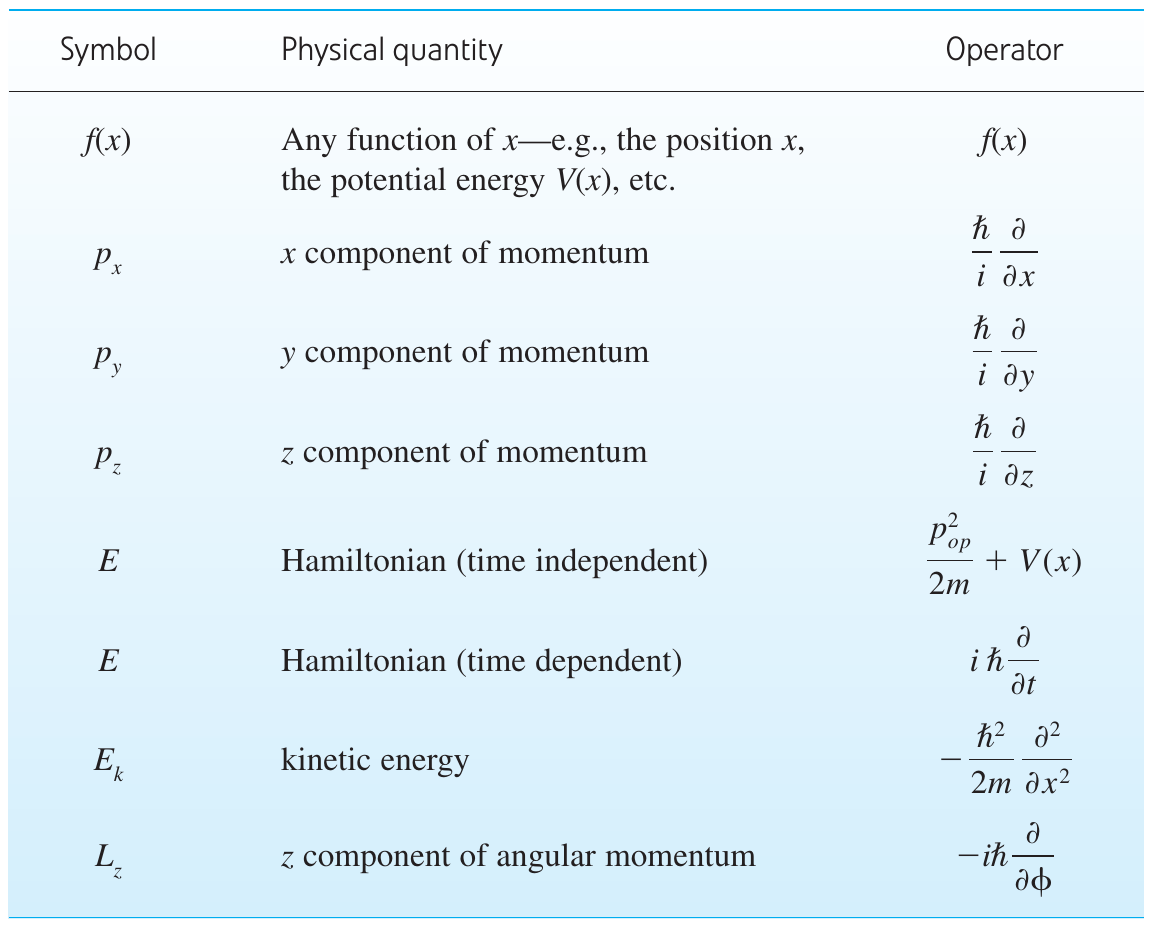
\includegraphics[width=9cm]{figuras/fig17}
  \end{figure}
\end{frame}

%%%%%%%%%%%%%%%%  SLIDE 14 %%%%%%%%%%%%%%%%%%%%%%%%%%

\begin{frame}
  \frametitle{Exemplo - Poço infinito}
  \begin{columns}[c]

  \column{5cm}
  
  \begin{figure}
    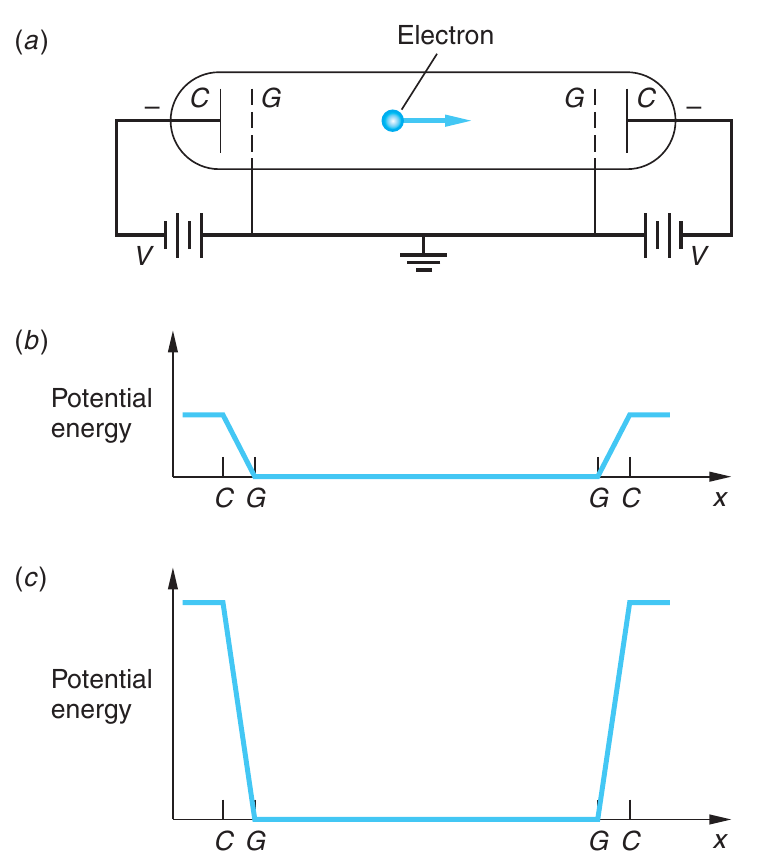
\includegraphics[width=5cm]{figuras/fig18a}
  \end{figure}
  
  \column{5cm}
  
  \begin{figure}
    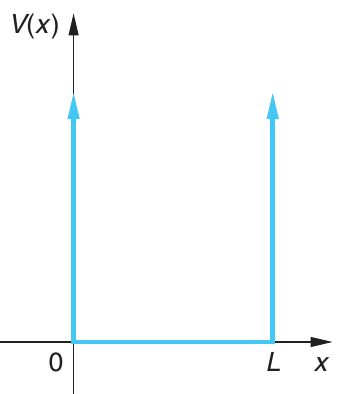
\includegraphics[width=3cm]{figuras/fig18b}
  \end{figure}
  
  \fontsize{10pt}{11pt}\selectfont
  \[
    V(x) = \begin{cases}
      0 & 0< x < L\\
      \infty & 0 \geq x \wedge x\geq L
    \end{cases}
  \]
  
  
  \end{columns}
\end{frame}

%%%%%%%%%%%%%%%%  SLIDE 15 %%%%%%%%%%%%%%%%%%%%%%%%%%

\begin{frame}
  \frametitle{Exemplo - Poço infinito}  
  \fontsize{8.5pt}{11pt}\selectfont
  
  Fora da caixa, $V(x) = \infty \Rightarrow \phi(x) = 0$. Dentro da caixa $V(x) = 0$ então a equação de Schrödinger
  \[
   -\dfrac{h^2}{2m}\dfrac{d^2\psi}{dx^2}=E\psi
  \]
  a solução dessa EDO
  \[
   \phi(x) = C_1 \sin \left( \sqrt{\dfrac{2mE}{h^2}}x \right) + C_2 \cos\left( \sqrt{\dfrac{2mE}{h^2}}x \right)
  \]
  aplicando condições de contorno 
  \[
   \psi_n(x) = C_1 \sin \left( \dfrac{n\pi}{L}x \right)
  \]
  \[
   E_n = \dfrac{n^2h^2}{8m}
  \]

  Normalizando a função de onda
  \[
   \int_\infty^\infty \psi_n^*\psi_n\, dx= 1 \Rightarrow C_1 = \sqrt{\dfrac{2}{L}}
  \]
  \[
   \psi_n(x) = \sqrt{\dfrac{2}{L}} \sin \left( \dfrac{n\pi}{L}x \right)
  \]
  
\end{frame}


%%%%%%%%%%%%%%%%  SLIDE 16 %%%%%%%%%%%%%%%%%%%%%%%%%%

\begin{frame}
  \frametitle{Exemplo - Poço infinito}  
  \fontsize{9pt}{11pt}\selectfont
  
  \begin{align*}
    \langle x \rangle& = \int_0^L \psi_n^* x \psi_n\,dx\\
              &= \dfrac{2}{L}\int_0^L x\sin^2 \left( \dfrac{n\pi}{L}x \right)\,dx\\
              &=\dfrac{1}{L}\int_0^L x\, dx - \dfrac{1}{L}\int_0^L x\cos\left( \dfrac{2n\pi}{L}x \right)\,dx\\
              &=\dfrac{1}{L}\int_0^L x\, dx - \left. \dfrac{1}{4n\pi}x\sin\left( \dfrac{2n\pi}{L}x \right) \right|_0^L + \dfrac{1}{4n\pi}\int_0^L\sin\left( \dfrac{2n\pi}{L}x \right)\,dx\\
            &=\dfrac{1}{2L}\left. x^2\right|_0^L - \left. \dfrac{1}{4n\pi}x\sin\left( \dfrac{2n\pi}{L}x \right) \right|_0^L + \dfrac{L}{8n^2\pi^2}\int_0^{2n\pi}\sin u\,du\\
            &= \dfrac{L}{2} - \dfrac{L}{4n\pi}\sin\left(2n\pi\right)+\dfrac{L}{8n^2\pi^2}\left[ 1 -\cos\left( 2n\pi \right) \right]\\
            &= L/2
  \end{align*}
  
\end{frame}



%%%%%%%%%%%%%%%%  SLIDE 17 %%%%%%%%%%%%%%%%%%%%%%%%%%

\begin{frame}
  \frametitle{Exemplo - Poço infinito}  
  \fontsize{8pt}{11pt}\selectfont
  
  Qual é a probabilidade de encontrar o elétron entre $x=0$ e $x=L/3$?
  \begin{columns}[c]
  
      \column{5cm}
        \fontsize{7pt}{11pt}\selectfont
      \begin{align*}
        \langle x \rangle &=\int_{0}^{L/3}\psi_{n}^{*}x\psi_{n}\,dx\\
            &=\dfrac{2}{L}\int_{0}^{L/3}x\sin^{2}\left(\dfrac{n\pi}{L}x\right)\,dx\\
            &=\dfrac{1}{L}\int_{0}^{L/3}x\,dx-\dfrac{1}{L}\int_{0}^{L/3}x\cos\left(\dfrac{2n\pi}{L}x\right)\,dx\\&=\dfrac{1}{L}\int_{0}^{L/3}x\,dx-\left.\dfrac{1}{2n\pi}x\sin\left(\dfrac{2n\pi}{L}x\right)\right|_{0}^{L/3}+\\
            &\dfrac{1}{2n\pi}\int_{0}^{L/3}\sin\left(\dfrac{2n\pi}{L}x\right)\,dx\\
            &=\dfrac{1}{2L}\left.x^{2}\right|_{0}^{L/3}-\left.\dfrac{1}{2n\pi}x\sin\left(\dfrac{2n\pi}{L}x\right)\right|_{0}^{L/3}+\\
            & \dfrac{L}{4n^{2}\pi^{2}}\int_{0}^{2n\pi/3}\sin u\,du\\
            &=\dfrac{L}{18}-\dfrac{L}{6n\pi}\sin\left(\dfrac{2}{3}n\pi\right)+\\
            &\dfrac{L}{4n^{2}\pi^{2}}\left[1-\cos\left(\dfrac{2}{3}n\pi\right)\right]
      \end{align*}
      
      \column{5cm}
        \vspace*{-0.6cm}
        \begin{figure}
          \hspace{-1.25cm}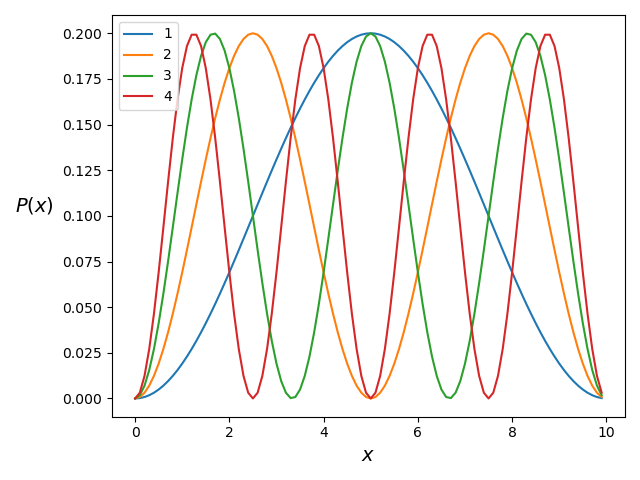
\includegraphics[width=4.5cm]{figuras/fig17c}
        \end{figure}
        \vspace*{-0.75cm}
        \begin{figure}
          \hspace{-1.25cm}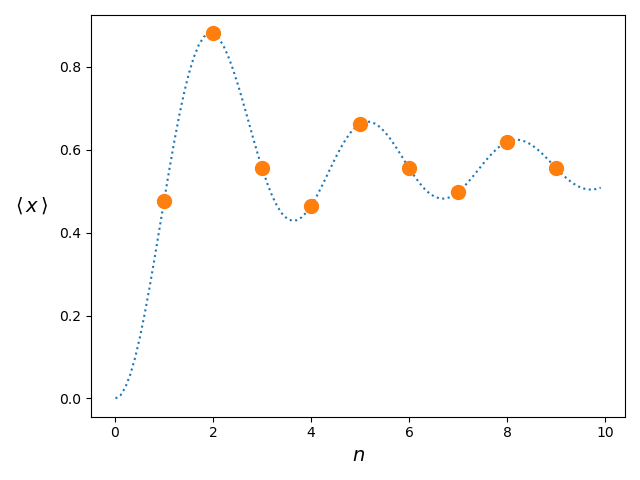
\includegraphics[width=4.5cm]{figuras/fig17b}
        \end{figure}
        \vspace*{-0.6cm}
        \href{https://www.st-andrews.ac.uk/physics/quvis/simulations_html5/sims/infwell1d/infwell1d.html}{\color{blue} Simulação no QuVis}
    \end{columns}
  
\end{frame}


%%%%%%%%%%%%%%%%  SLIDE 18 %%%%%%%%%%%%%%%%%%%%%%%%%%

\begin{frame}
  \frametitle{Exemplo - Poço infinito}  
  \fontsize{9pt}{11pt}\selectfont
  
    \begin{align*}
            \langle p_x \rangle & = \dfrac{\hbar}{i}\int_0^L \psi_n^* \dfrac{\partial\;}{\partial x} \psi_n\,dx\\
            &= \dfrac{2\hbar}{iL}\int_0^L \sin \left( \dfrac{n\pi}{L}x \right)\dfrac{\partial\;}{\partial x}\left[ \sin \left( \dfrac{n\pi}{L}x \right) \right]\,dx\\
            &= \dfrac{2\hbar}{iL}\dfrac{n\pi}{L}\int_0^L \sin \left( \dfrac{n\pi}{L}x \right)\dfrac{\partial\;}{\partial x}\cos \left( \dfrac{n\pi}{L}x \right)\,dx\\
            &= 0
          \end{align*}
  
\end{frame}

%%%%%%%%%%%%%%%%  SLIDE 19 %%%%%%%%%%%%%%%%%%%%%%%%%%

\begin{frame}
  \frametitle{Exemplo - Poço infinito}  
  \fontsize{8.5pt}{11pt}\selectfont
  
  \begin{columns}[c]

  \column{5cm}
    \begin{align*}
            \langle p_x^2 \rangle& = \dfrac{\hbar}{i}\int_0^L \psi_n^* \left( \dfrac{\hbar}{i}\dfrac{\partial\;}{\partial x} \right)^2 \psi_n\,dx\\
            \left( \dfrac{\hbar}{i} \dfrac{\partial\;}{\partial x} \right)^2 \psi_n &= -\hbar^2\left( \dfrac{\partial\;}{\partial x} \right) \left( \dfrac{\partial\;}{\partial x} \right)\psi_n\\
            &= -\hbar^2\dfrac{2}{L}\left( \dfrac{\partial\;}{\partial x} \right) \left( \dfrac{\partial\;}{\partial x} \right)\sin\left( \dfrac{2n\pi}{L}x \right)\\
            &= -\hbar^2\dfrac{2}{L}\dfrac{n\pi}{L}\left( \dfrac{\partial\;}{\partial x} \right)\cos \left( \dfrac{n\pi}{L}x \right)\\
            &= \hbar^2\dfrac{n^2\pi^2}{L^2}\dfrac{2}{L}\sin \left( \dfrac{n\pi}{L}x \right)\\
            &= \hbar^2\dfrac{n^2\pi^2}{L^2}\psi_n
          \end{align*}
  \column{5cm}
          assim
          \begin{align*}
            \langle p_x^2 \rangle& = \hbar^2\dfrac{n^2\pi^2}{L^2}\int_0^L \psi_n^*\psi_n\,dx\\
            & = \dfrac{n^2\hbar^2\pi^2}{L^2}\\
            & = \dfrac{n^2h^2}{4L^2}
          \end{align*}
  \end{columns}
\end{frame}

%%%%%%%%%%%%%%%%  SLIDE 20 %%%%%%%%%%%%%%%%%%%%%%%%%%

\begin{frame}
  \frametitle{Exemplo - Poço infinito}  
  \fontsize{9pt}{11pt}\selectfont
  
  \begin{itemize}
   \item Devemos ter claro o nosso resultado, para uma dada função de onda $\psi_n$, temos uma energia $E_n$ associada. Isso significa que se nos preparamos o sistema de forma tal que $\Psi = \psi_n$ então o resultado da medida será $E_n$ e isso acontecerá sempre que nos preparemos o sistema nesse estado.
   \item As funções de onda que a partícula pode assumir não se restringem a $\psi_n$, é possível preparar o sistema em estados que são uma combinação linear dos estados $\psi_n$.
   \item  Se preparamos o sistema numa combinação de estados, por exemplo  $\Psi = \dfrac{1}{\sqrt{2}}\left( \psi_1 + \psi_2\right)$ não mas teremos certeza sobre o valor de energia que resultará numa medida, só sabemos que teremos uma probabilidade de 0,5 de obter $E_1$ e 0,5 de obter $E_2$
   \item Note que não obtivemos $\psi_0$, ou seja, o menor valor de energia que o sistema pode assumir é $E_1$, isso está relacionado ao fato de que se a partícula não pode ter zero energia (cinética) pois isso implicaria que estaria parada em algum lugar e com momento zero, isso seria uma violação ao principio de incerteza. Este tipo de comportamento (energia de ponto zero) acontece em todos os sistemas confinados.
  \end{itemize}
  
\end{frame}



%%%%%%%%%%%%%%%%  SLIDE 21 %%%%%%%%%%%%%%%%%%%%%%%%%%

\begin{frame}
  \frametitle{Exemplo - Poço Finito}
  
  \fontsize{10pt}{11pt}\selectfont
  \begin{columns}
    \column{0.6\linewidth}  
  $
    V(x) = \left\{ \begin{array}{lll}
            V_0 & 0\leq x &\text{região I}\\
            0 & 0 < x < 0 &\text{região II}\\
            V_0 & 0\geq x &\text{região I}
           \end{array}\right.
  $
  \column{0.4\linewidth}
  \hspace*{-0.5cm}\centering 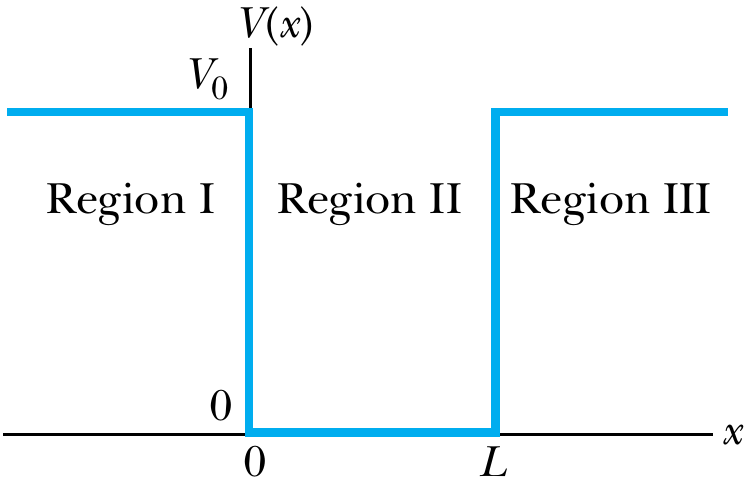
\includegraphics[height=3.cm]{figuras/fig20b}
  \end{columns}
  
  \vspace{0.25cm}
  \begin{columns}
    \column{0.5\linewidth} 
    Para as regiões I e III a equação de Schrödinger assume a forma
  \column{0.5\linewidth}
    \[
      -\dfrac{\hbar}{2m}\dfrac{1}{\psi}\dfrac{d^2\psi}{dx^2}=E-V_0
    \]
  \end{columns}
  
  
  \vspace{0.25cm}
  \begin{columns}
    \column{0.5\linewidth} 
    Utilizando $\alpha^2=2m\left( V_0 - E \right)/\hbar$, podemos reescreve
  \column{0.5\linewidth}
  \hspace*{1cm}
    \[
      d^2\psi / dx^2 = \alpha ^2\psi
  \]
  \end{columns}  
  
  \vspace{0.25cm}
  \begin{columns}
    \column{0.5\linewidth} 
    Levando em consideração o fato de que $\psi\to 0$ para $x\leq 0$ e $x \geq L$, propomos como solução
  \column{0.5\linewidth}
  
  \[
      \begin{array}{lll}
        \psi_I(x) = Ae^{\alpha x}  & 0\leq x &\text{região I}\\
        \psi_{II}(x) = Be^{-\alpha x} & x \geq L &\text{região III}
           \end{array}
  \]
  \end{columns}
  
\end{frame}




%%%%%%%%%%%%%%%%  SLIDE 21 %%%%%%%%%%%%%%%%%%%%%%%%%%

\begin{frame}
  \frametitle{Exemplo - Poço Finito}
  \fontsize{9pt}{11pt}\selectfont

  Dentro do poço de potencial, onde $V(x) = 0$, a equação da onda é
  \[
   d^2\psi / dx^2 = -k^2\psi,\qquad k=\sqrt{(2mE)/\hbar^2}
  \]
  como solução propomos
  \[
   \psi_{II}(x) = Ce^{ikx} + De^{-ikx},\qquad 0< x < L
  \]
  As condições de contorno que devem ser satisfeitas são
  \[
   \psi_I(0) = \psi_{II}(0)\quad\text{e}\quad \psi_{II}(L) = \psi_{II}(L)
  \]
  
  \begin{columns}
    \column{0.35\linewidth} 
    O que resulta numa função de onda continua nas fronteiras.\newline\newline
    Note que $\psi$ não é zero fora da caixa
    \column{0.65\linewidth}
    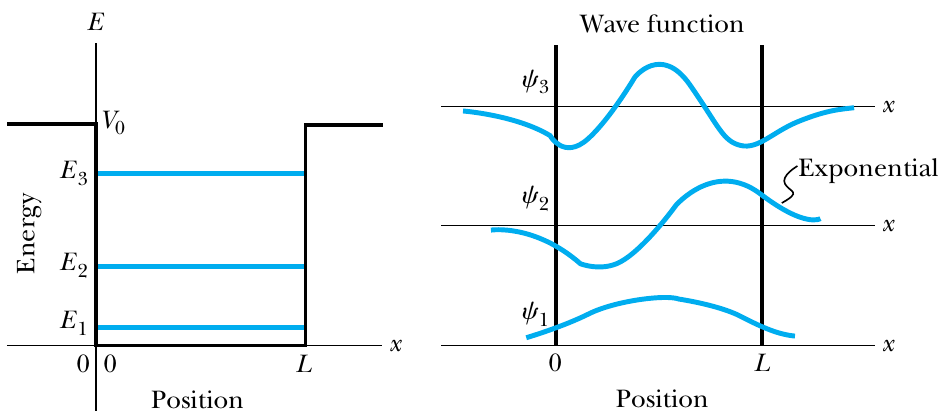
\includegraphics[height=3.5cm]{figuras/fig21}
  \end{columns}  

  
\end{frame}


%%%%%%%%%%%%%%%%  SLIDE 22 %%%%%%%%%%%%%%%%%%%%%%%%%%

\begin{frame}
  \frametitle{Exemplo - Poço Finito}
  \fontsize{9pt}{11pt}\selectfont
  
  \begin{center}
  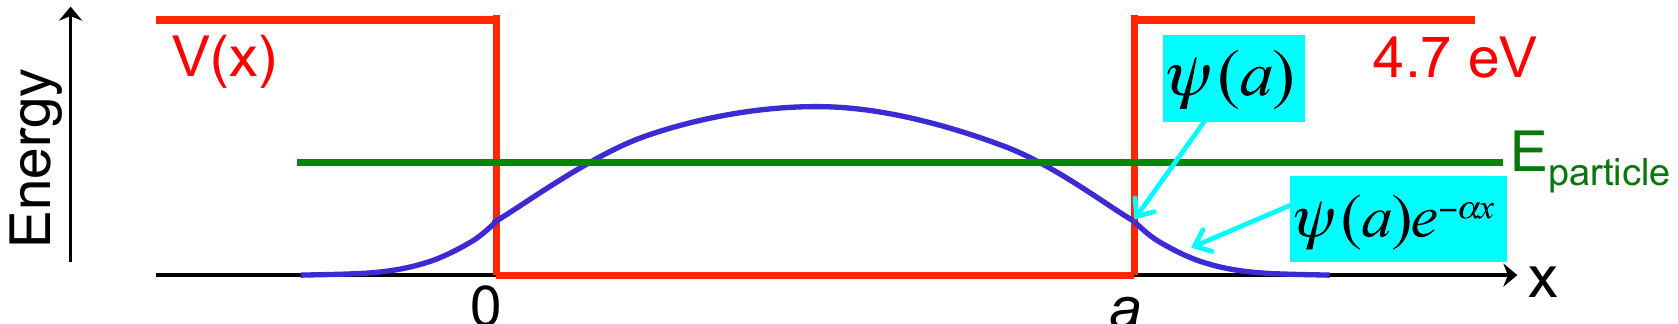
\includegraphics[height=2cm]{figuras/fig22b} 
  \end{center}

  \begin{columns}
  
    \column{0.65\linewidth}
    Observe que
  \[
   \lambda = \dfrac{1}{\alpha} = \dfrac{\hbar}{\sqrt{2m\left(V_0 - E\right)}}
  \]
  é uma medida da profundidade de penetração dentro da região proibida.  Em essa distância $\psi (x)$ se reduz por um fator $1/e$.\\
  
  Como exemplo consideremos um elétron com $4,7\,eV$, nesse caso a profundidade de penetração é só de $10^{-10}m$ (tamanho de um átomo)
    
    \column{0.35\linewidth}
    
      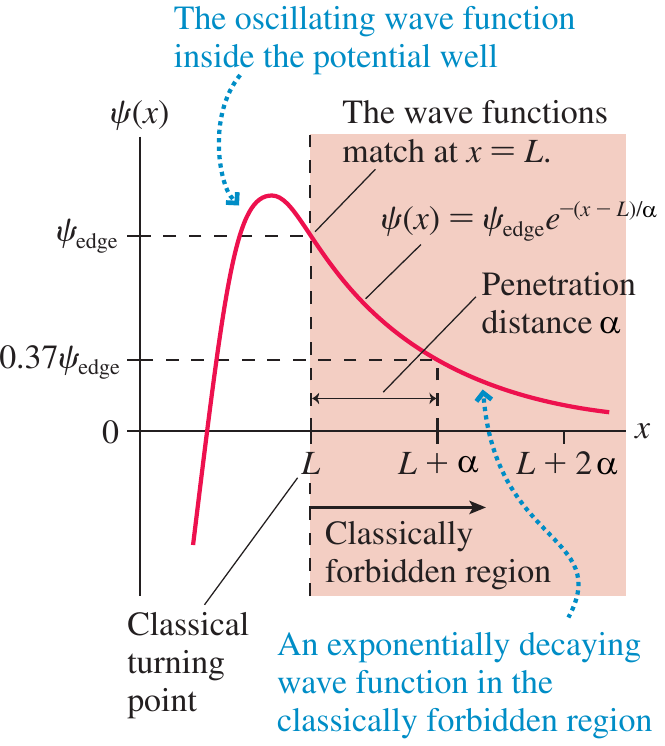
\includegraphics[width=4cm]{figuras/fig22c}
  \end{columns} 
  
\end{frame}



%%%%%%%%%%%%%%%%  SLIDE 23 %%%%%%%%%%%%%%%%%%%%%%%%%%

\begin{frame}
  \frametitle{Exemplo - Comparação do Poço Infinito com o Finito}
  \fontsize{10pt}{11pt}\selectfont
  
   \centering 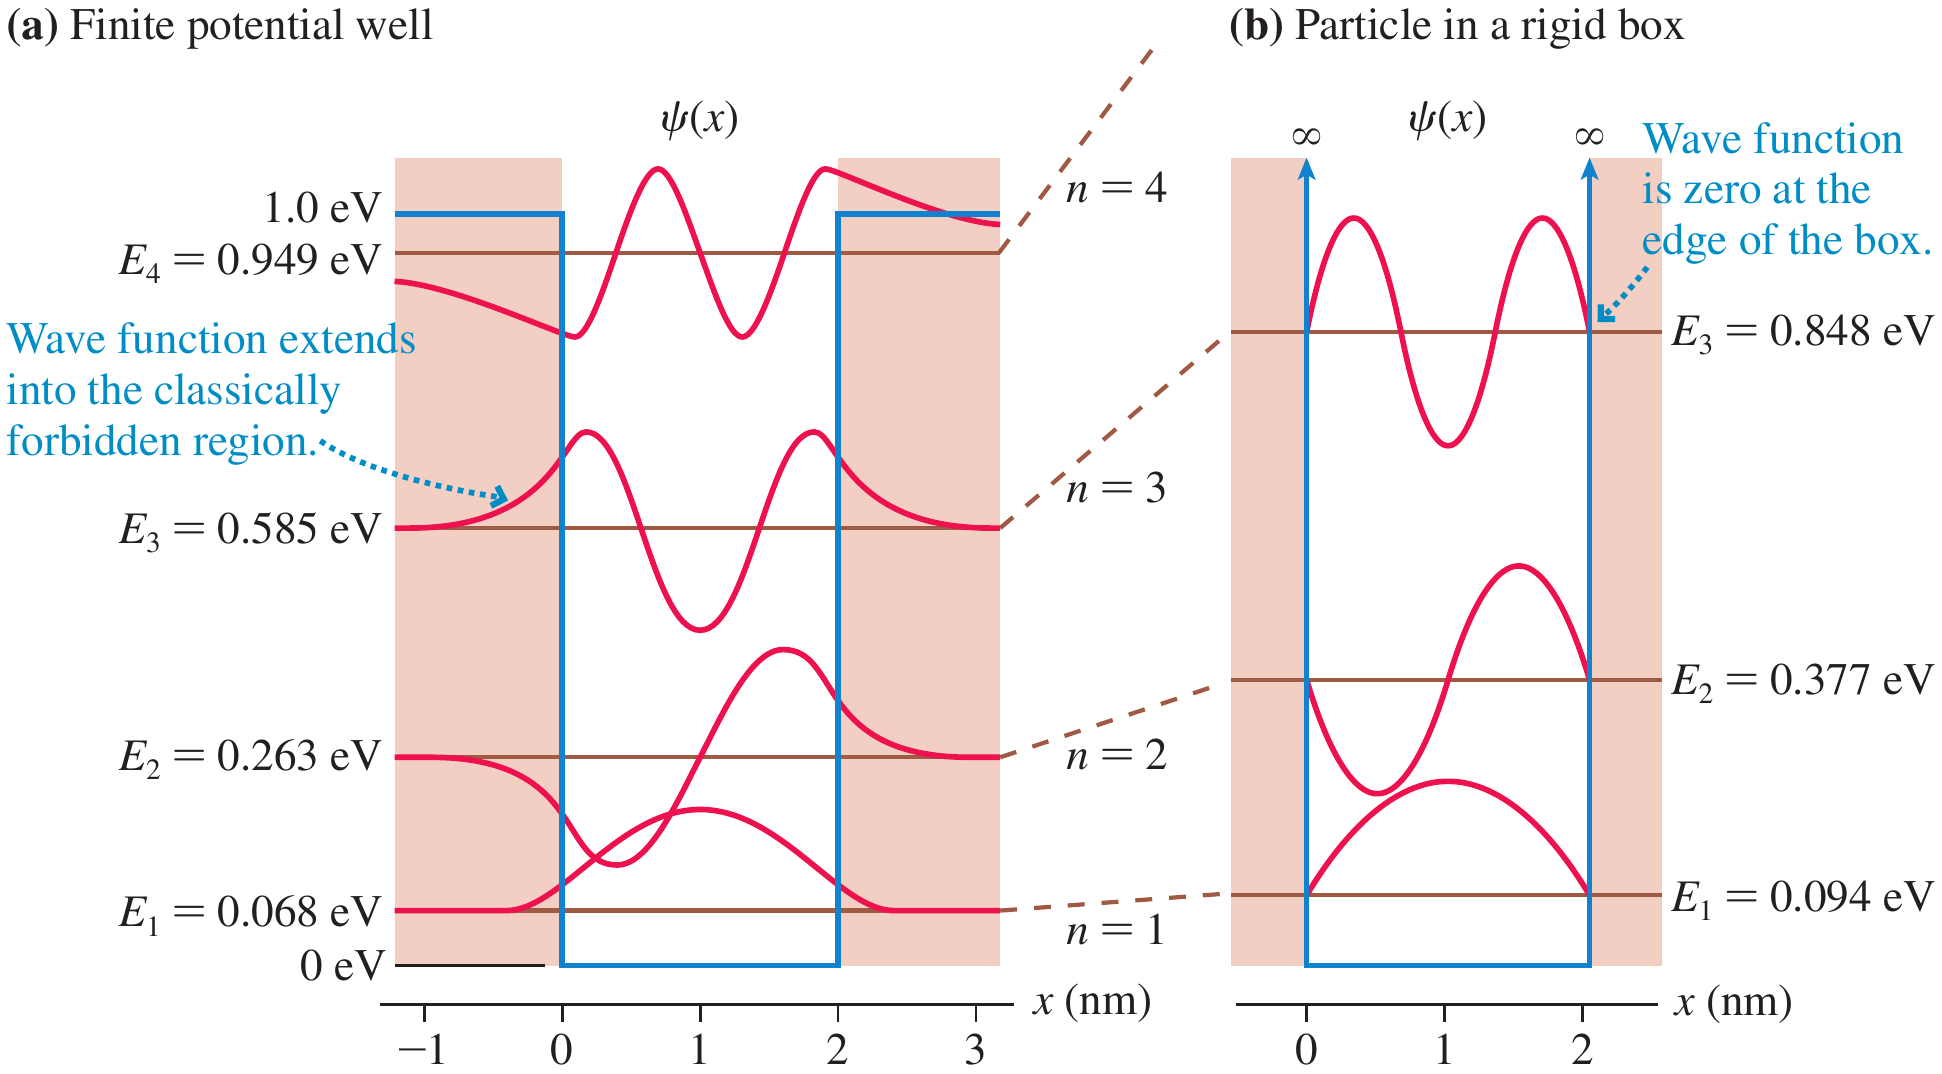
\includegraphics[height=6.5cm]{figuras/fig23}
 
\end{frame}

%%%%%%%%%%%%%%%%  SLIDE 24 %%%%%%%%%%%%%%%%%%%%%%%%%%

\begin{frame}
  \frametitle{Exemplo - LASER de estado sólido\\}
  
  \fontsize{9pt}{11pt}\selectfont
  \begin{columns}
    \column{0.6\linewidth}
    
      {\centering \vspace*{-1cm}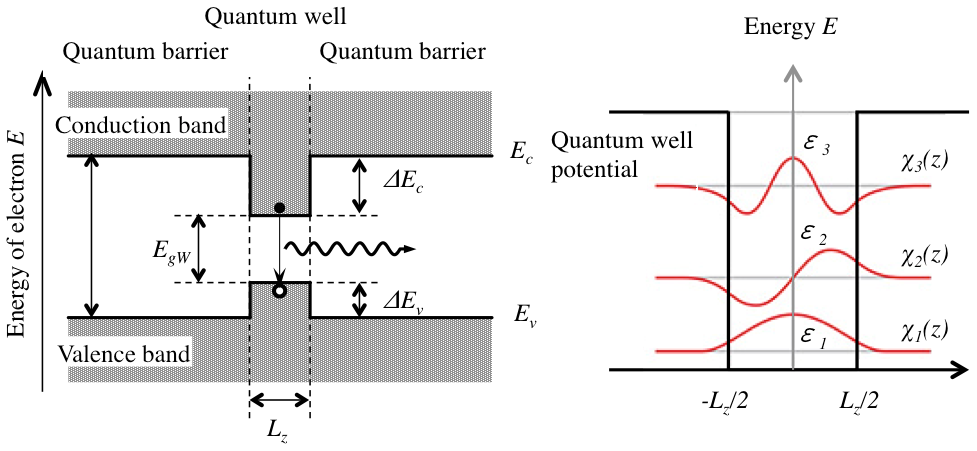
\includegraphics[width=7cm]{figuras/fig25}}
      \begin{align*}
        v_{rms}&=\sqrt{\dfrac{3k_bT}{m}} \approx 1\times 10^{5}m/s\\
        \lambda &\approx \dfrac{h}{mv_{rms}}\approx 7\,nm
      \end{align*}
      {Efeitos quânticos acontecem para sistemas da ordem de 7 nm ou menos (na real até 100 nm ou menos)\\
      
      Poços quânticos permitem construir ``átomos'' artificiais, isto é, ter controle nos nível de energia.\\}
    \column{0.4\linewidth}
    
    {\centering \vspace*{-0.5cm}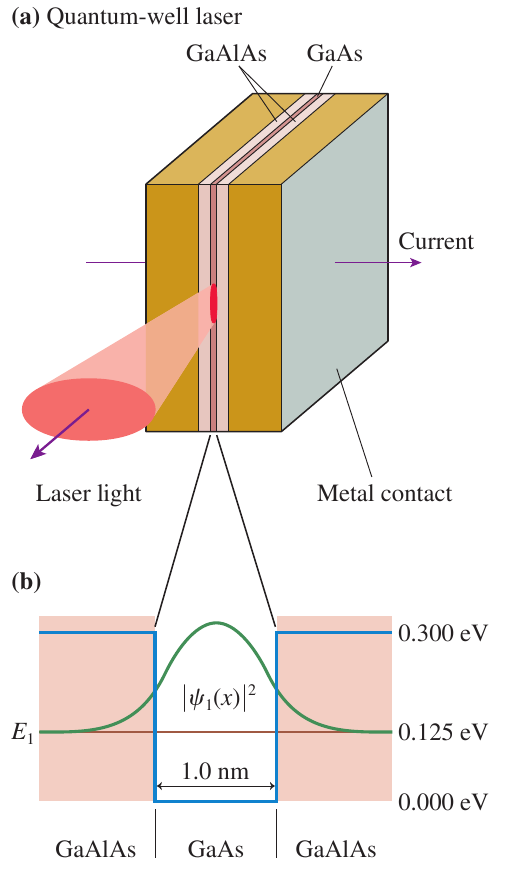
\includegraphics[height=6.5cm]{figuras/fig24}}
    
    \fontsize{6pt}{11pt}\selectfont
    No poço acima, $GaAlAs$, $GaAs$, $GaAlAs$, $V_0 = 0,3 eV$ e $L=1,0 nm$ resulta em um único nível de energia.
  \end{columns}
 
\end{frame}
  
%%%%%%%%%%%%%%%%  SLIDE 25 %%%%%%%%%%%%%%%%%%%%%%%%%%

\begin{frame}
  \frametitle{Exemplo - Núcleo atômico\\}
  
  \fontsize{9pt}{11pt}\selectfont
  \vspace*{-1.5cm}
  \begin{columns}
    \column{0.5\linewidth}
    
    Modelemos o núcleo com $L=8$  (próximo ao argon ou potássio) e $V_0=50 MeV$. Consideremos um nêutron exitado em $n=3$, da figura vemos que
    \begin{align*}
      E_{\text{fóton}} &= E_3 - E_1\\
      &= 19,1\,MeV     
    \end{align*}

    de onde
    \[
     \lambda = \dfrac{c}{f} = \dfrac{hc}{E_{\text{fóton}}}=6,5\times 10^{-5}\,nm
    \]
    o que corresponde a fótons na região da radiação Gamma.
    
    \column{0.5\linewidth}
    
    {\centering \vspace*{0.5cm}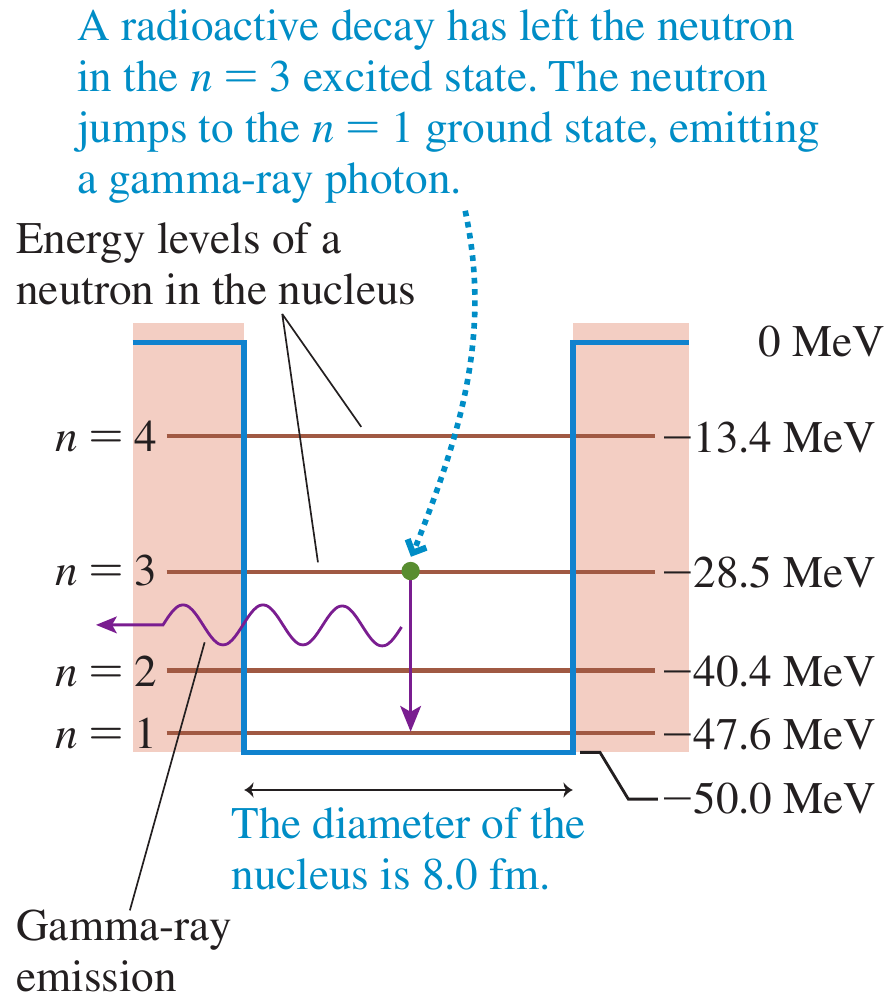
\includegraphics[height=6.5cm]{figuras/fig26}}
    
    \fontsize{6pt}{11pt}\selectfont
      Três dos quatro níveis energéticos permitidos dentro de um poço de potencial nuclear
  \end{columns}
   

\end{frame}


  
%%%%%%%%%%%%%%%%  SLIDE 26 %%%%%%%%%%%%%%%%%%%%%%%%%%

\begin{frame}
  \frametitle{O oscilador harmônico Quântico}
  
  
  \fontsize{9pt}{11pt}\selectfont
  \begin{columns}
    
    \column{0.5\linewidth}
    
      Suponhamos $V(x) = \dfrac{1}{2}kx^2=\dfrac{1}{2}m\omega^2x^2$, então
      \[
       -\dfrac{h^2}{2m}\dfrac{\partial^2\psi}{\partial x^2}+\dfrac{1}{2}m\omega^2x^2 x=E\psi
      \]
      a qual pode ser resolvida e obtermos
      
      \[
       E_n = \left( n + \dfrac{1}{2} \right)\hbar \omega,\qquad n=0,\, 1,\, 2, \, \ldots
      \]
      de onde temos a energia de ponto zero dada por $E_0=\dfrac{1}{2} \hbar \omega$, enquanto que as funções de onda são dadas por
      
      \[
       \psi_n (x) = C_n e^{-m\omega x^2/2\hbar}H_n (x)
      \]
    \column{0.5\linewidth}
    
    {\centering 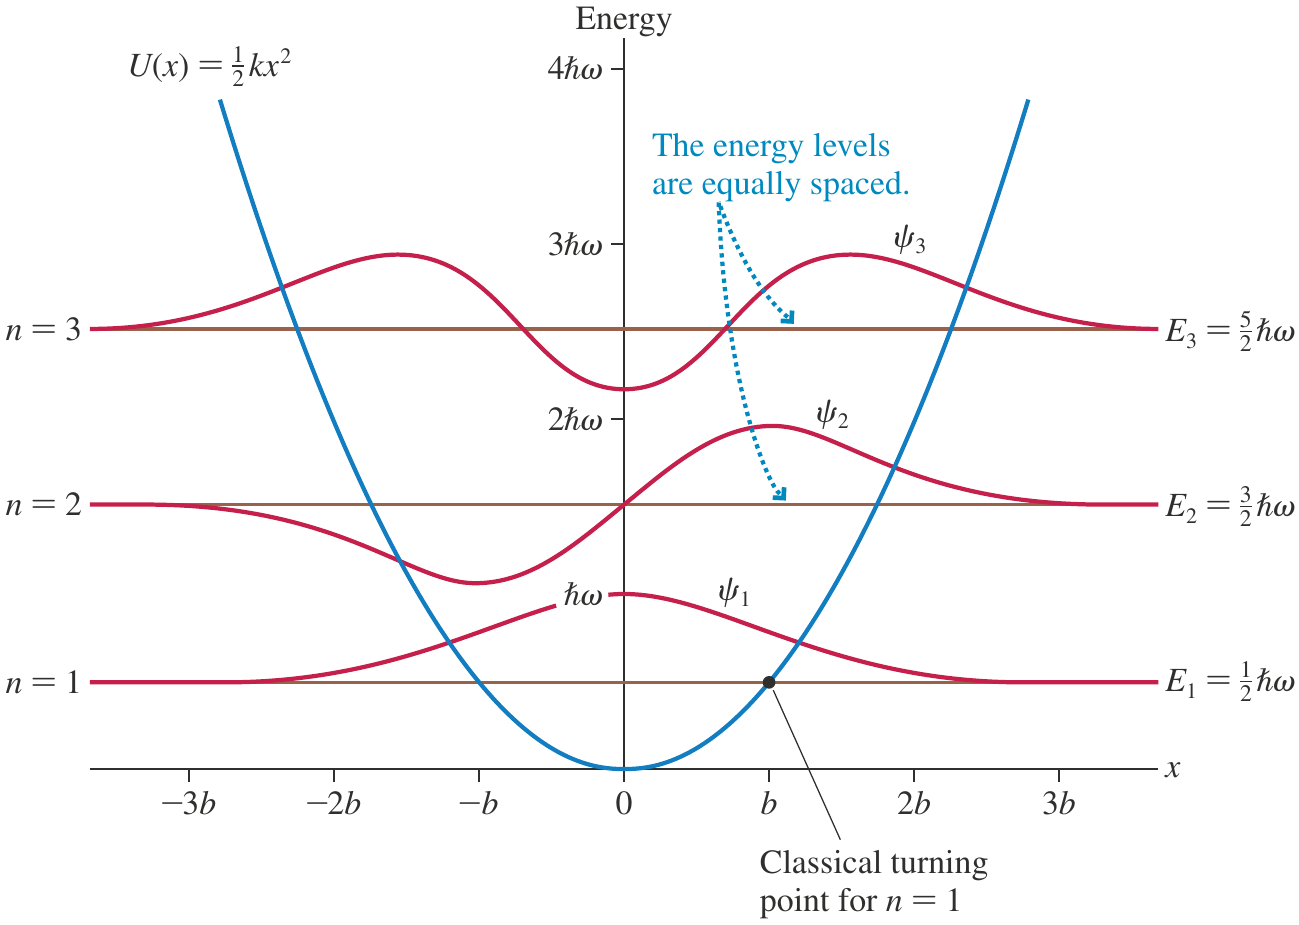
\includegraphics[height=4.cm]{figuras/fig27}}

    Pode ser mostrada a seguinte regra de seleção para as transições entre estados
    \begin{align*}
     \int_{-\infty}^{\infty} \psi_n\, x \, \psi_m\, dx=0\quad & \text{a menos que}\\
     &  n=m\pm 1
    \end{align*}

    
    ou $\Delta n = \pm 1$

      
  \end{columns}
\end{frame}


  
%%%%%%%%%%%%%%%%  SLIDE 27 %%%%%%%%%%%%%%%%%%%%%%%%%%

\begin{frame}
  \frametitle{O oscilador harmônico Quântico}
    \vspace{-0.25cm}
    \begin{minipage}[t][20ex][t]{\linewidth}
      \begin{center}
        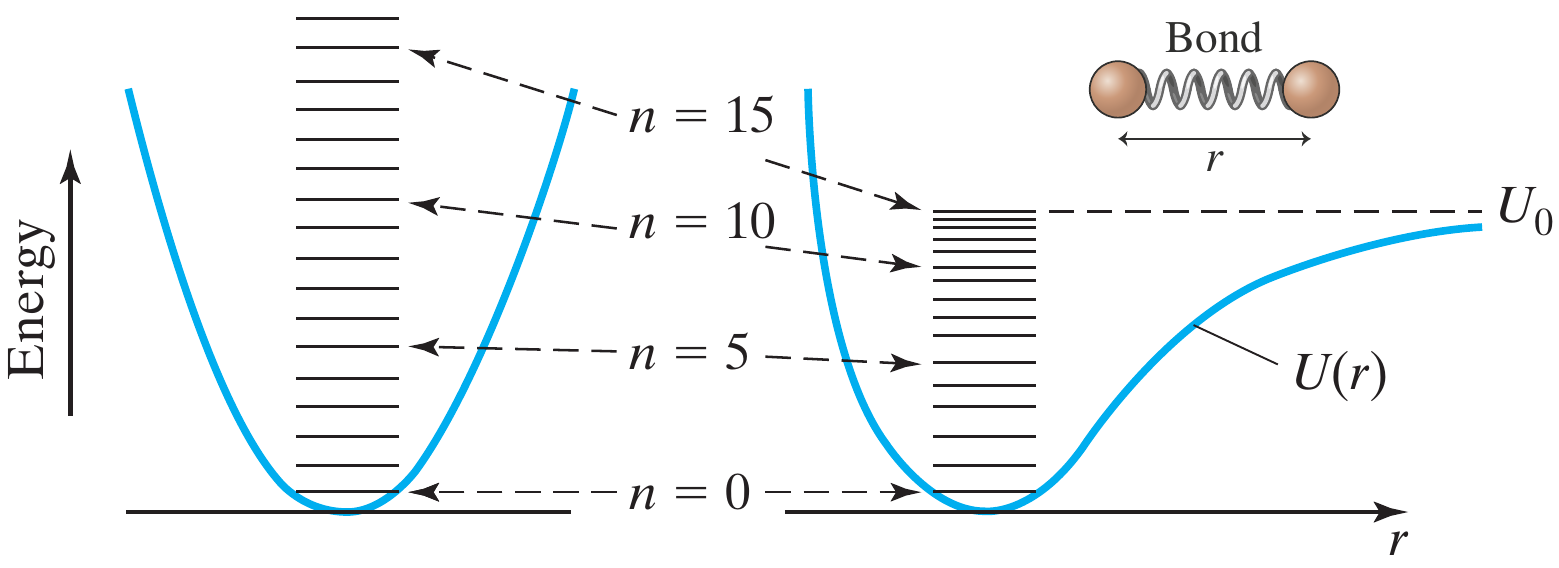
\includegraphics[height=3.25cm]{figuras/fig28}
      \end{center}
    \end{minipage}
    
    \vspace*{-1.5cm}
    \begin{minipage}[b][20ex][t]{\linewidth}
      \begin{columns}
        \column{0.5\linewidth}
        \fontsize{9pt}{11pt}\selectfont
        
        \vspace*{1.cm}        
        \begin{minipage}{\linewidth}
          Espectro de absorção da acetona. Acontece na região infravermelha. Temos duas transições correspondente a transições dos estados $1\to 2$, uma corresponde a vibração $C-CH_3$ em $\lambda = 3,3\,cm$, e outra $C=O$ em $\lambda = 5,8\,cm$
        \end{minipage}
        \column{0.5\linewidth}    
          \begin{center}
            \hspace*{-0.25cm}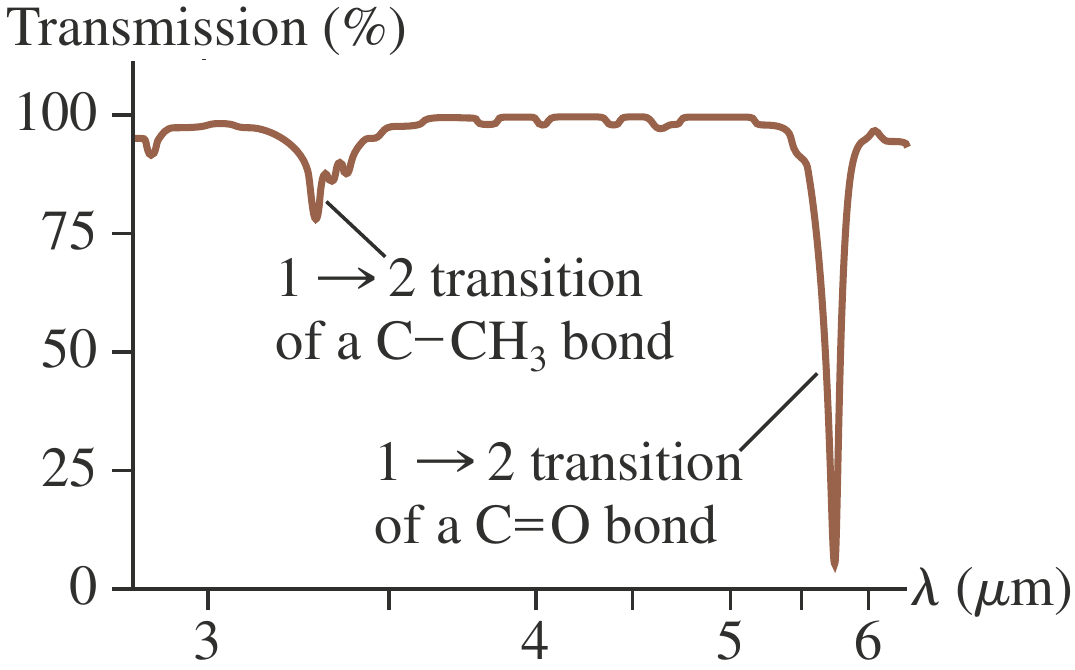
\includegraphics[height=4.cm]{figuras/fig29}
          \end{center}
      \end{columns}

    \end{minipage}

\end{frame}


  
%%%%%%%%%%%%%%%%  SLIDE 29 %%%%%%%%%%%%%%%%%%%%%%%%%%

\begin{frame}
  \frametitle{Exemplo - Ligação covalente\\}
  
  \fontsize{9pt}{11pt}\selectfont
  \vspace*{-1.5cm}
  \begin{columns}
    \column{0.6\linewidth}
    
    Uma aproximação ao átomo de hidrogênio é via um potencial quadrado com profundidade de $V_0=-24,2eV$ e $L=2a_B$. Essa escolha resulta em um primeiro estado exitado de $E_1=E_{0B}=-13,6eV$
    
    \column{0.4\linewidth}
    
    {\centering \vspace*{0.5cm}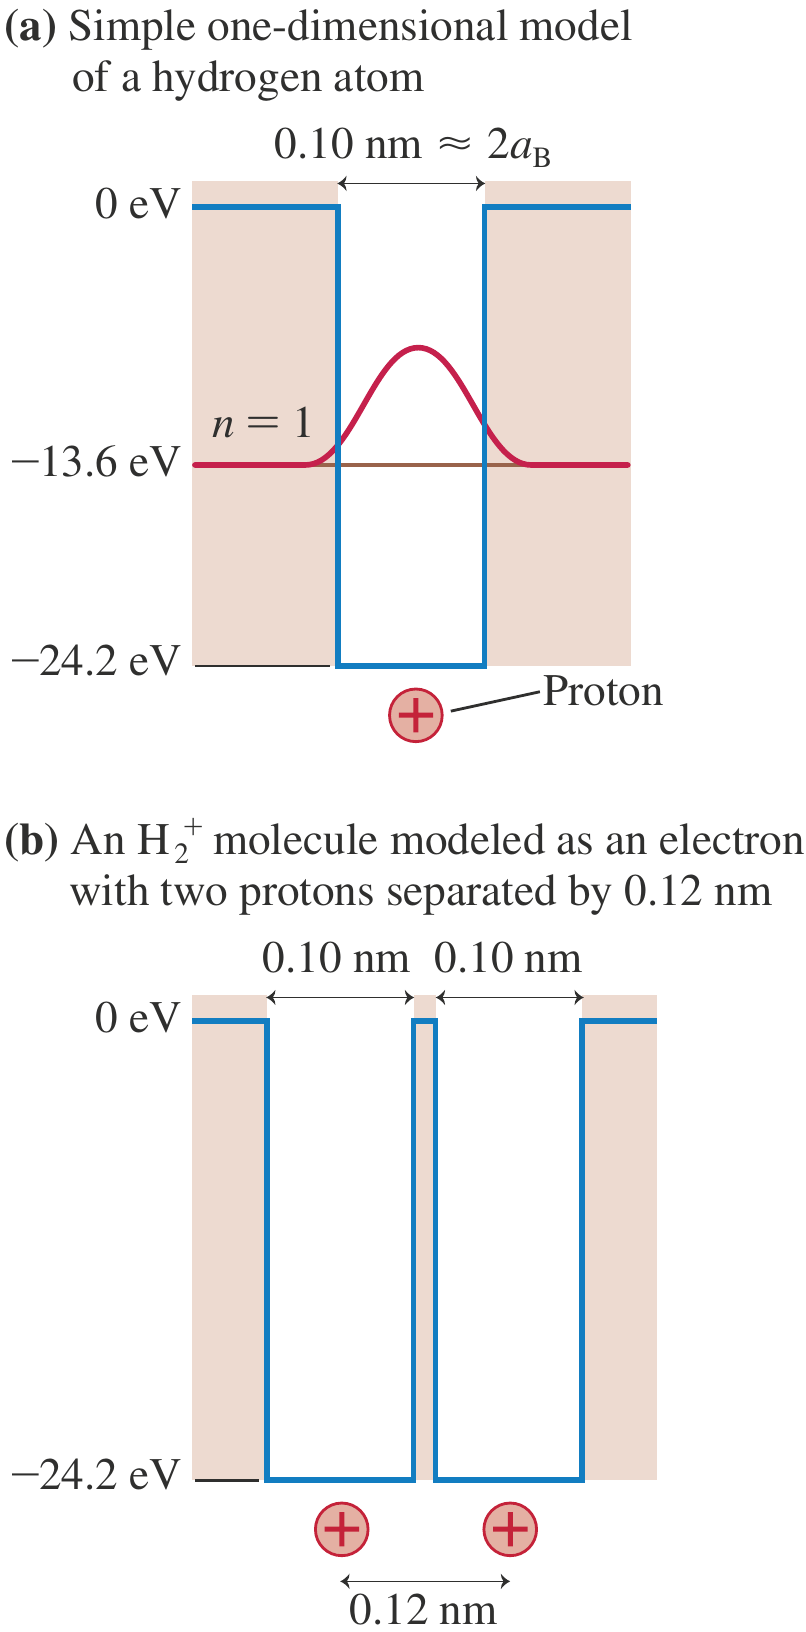
\includegraphics[height=7.5cm]{figuras/fig30}}
    
    \fontsize{6pt}{11pt}\selectfont
      
  \end{columns}
   

\end{frame}
  
%%%%%%%%%%%%%%%%  SLIDE 30 %%%%%%%%%%%%%%%%%%%%%%%%%%

\begin{frame}
  \frametitle{Exemplo - Ligação covalente\\}
  
  \fontsize{9pt}{11pt}\selectfont
  
   \begin{center}
     \vspace*{-1cm}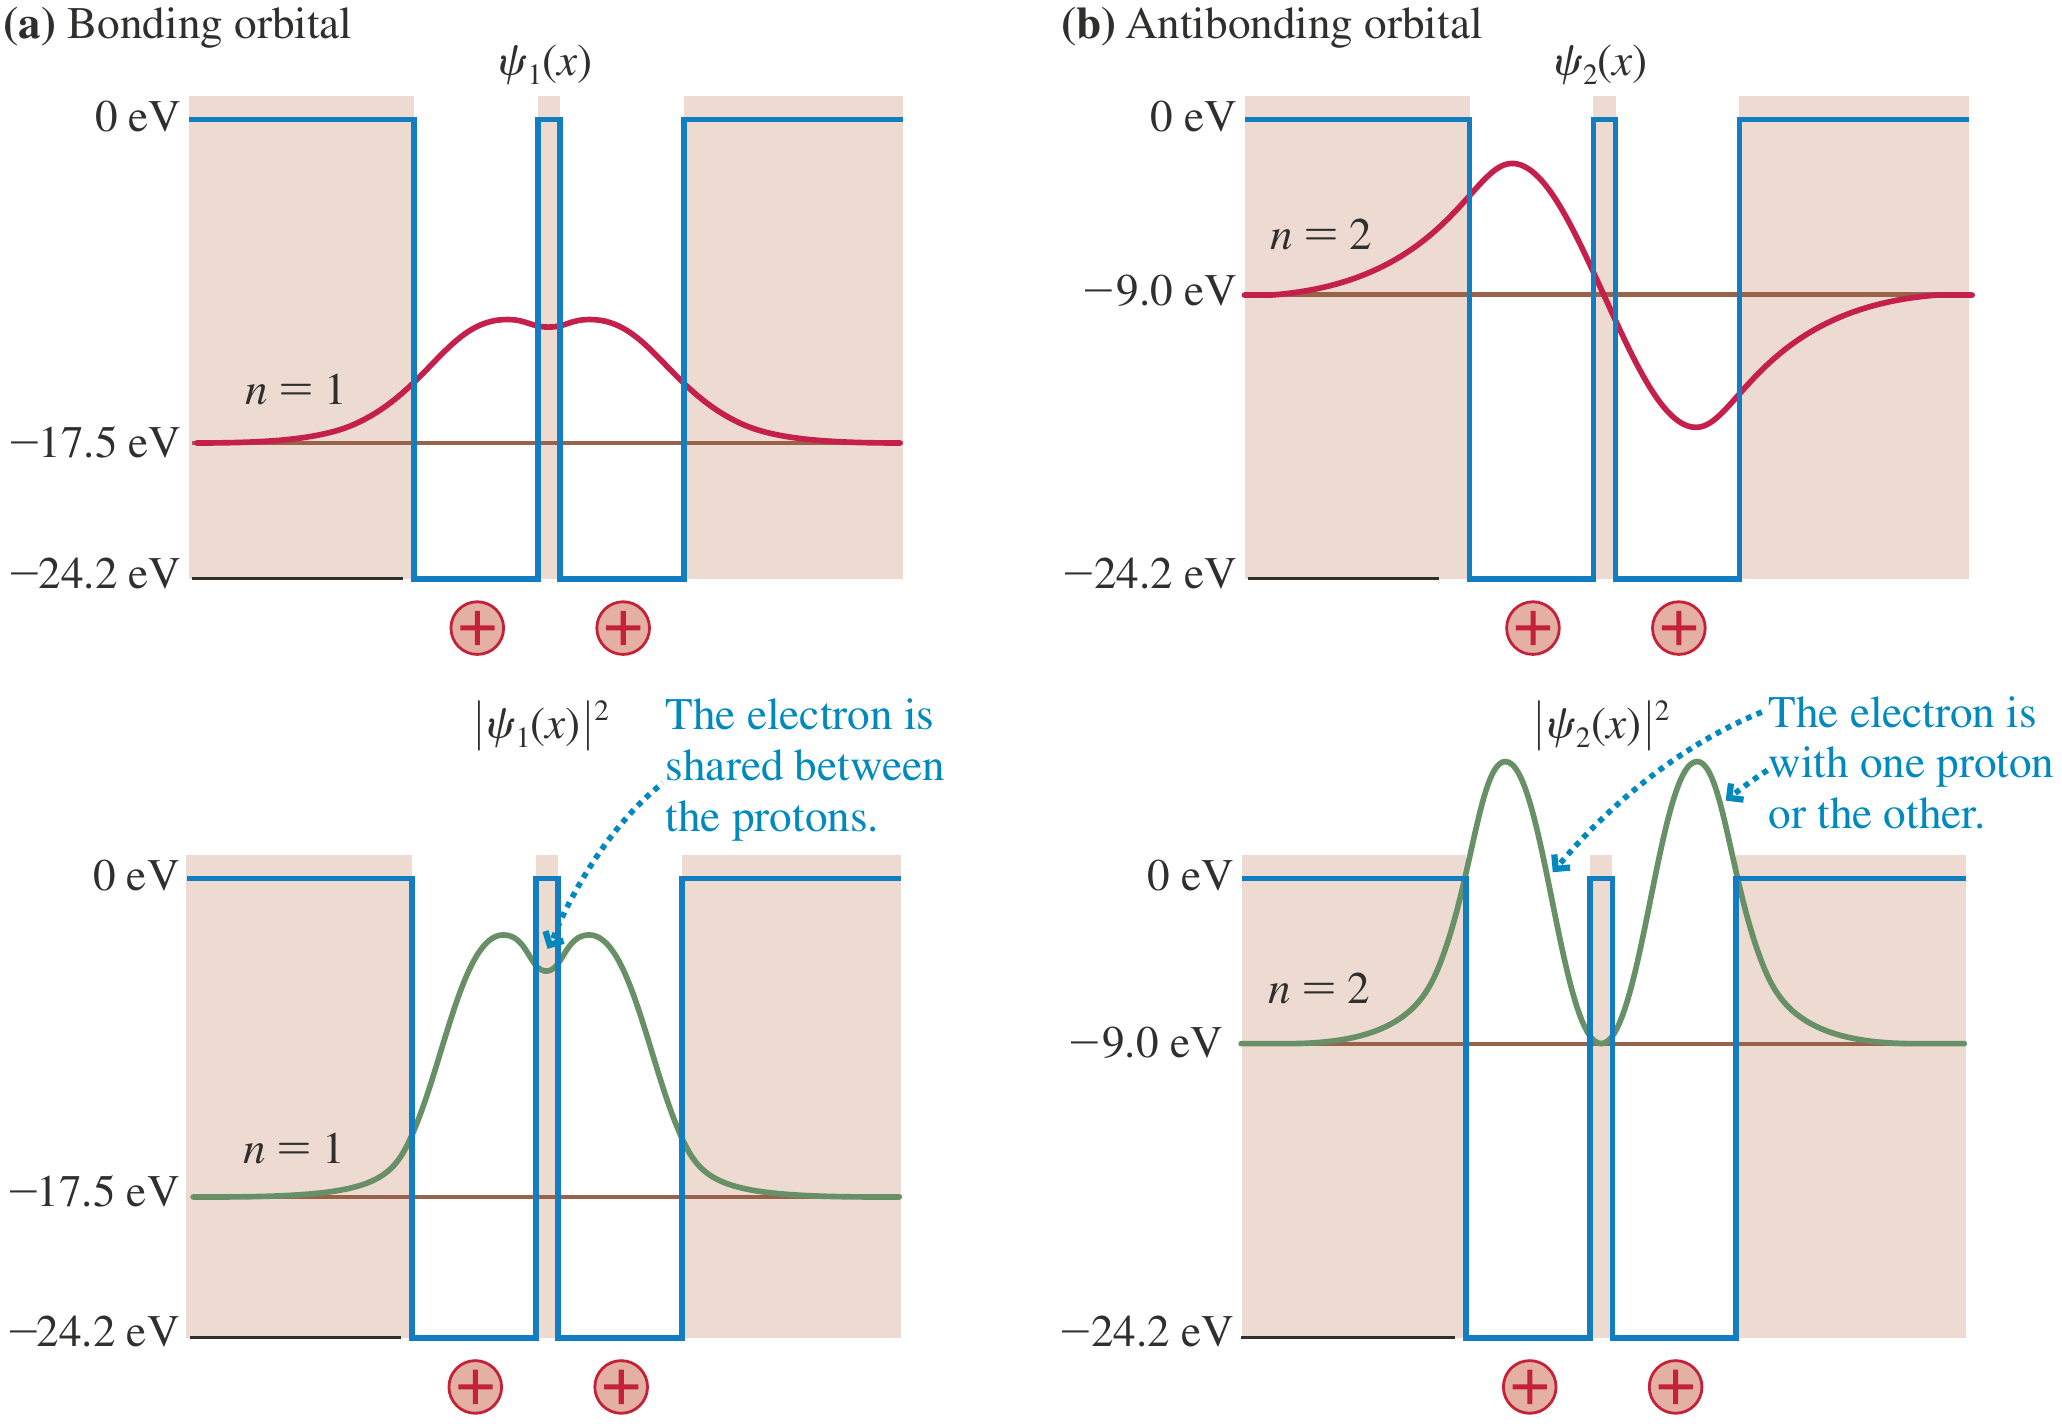
\includegraphics[height=5.5cm]{figuras/fig31}\vspace*{-0.5cm}
   \end{center}
   
    \[
     E_{mol} = E_{p-p}+E_{elec}= \left\{\begin{array}[0.8]{lcrcr}
                                   12,0 eV - 17,5eV &=& -5,5eV & \, &n=1\\ 
                                   12,0 eV - 9,0eV &=& +3,0eV & \, &n=2
                                 \end{array}\right.
    \]
  Note que a energia para $n=1$ é negativa (sistema ligado) enquanto que para $n=2$ é positivo (não ligado)
   

\end{frame}


  
%%%%%%%%%%%%%%%%  SLIDE 31 %%%%%%%%%%%%%%%%%%%%%%%%%%

\begin{frame}
  \frametitle{Barreira de Potencial}
  
  \fontsize{9pt}{11pt}\selectfont
  
    \begin{minipage}[t][20ex][t]{\linewidth}
      \begin{center}
        \vspace*{-1cm}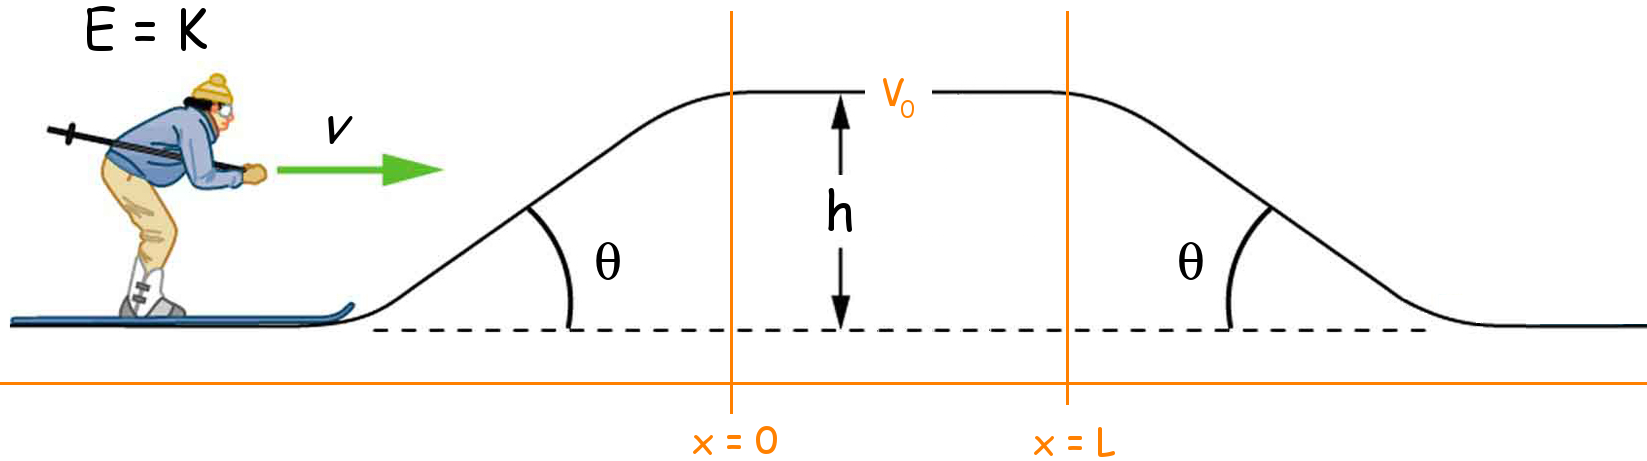
\includegraphics[height=3cm]{figuras/fig32}
      \end{center}
    \end{minipage}
    
    \vspace*{-1.cm}
    \begin{minipage}[b][20ex][t]{\linewidth}
      \begin{columns}
        \column{0.5\linewidth}
        \fontsize{9pt}{11pt}\selectfont
        
        \vspace*{1.cm}        
        \begin{minipage}{\linewidth}
           Considere uma partícula com energia $E$ se aproximando de uma barreira de potencial com altura $V_0$, sendo que qualquer outro lugar o potencial é zero.
        \end{minipage}
        
        \column{0.5\linewidth}    
          \begin{center}
            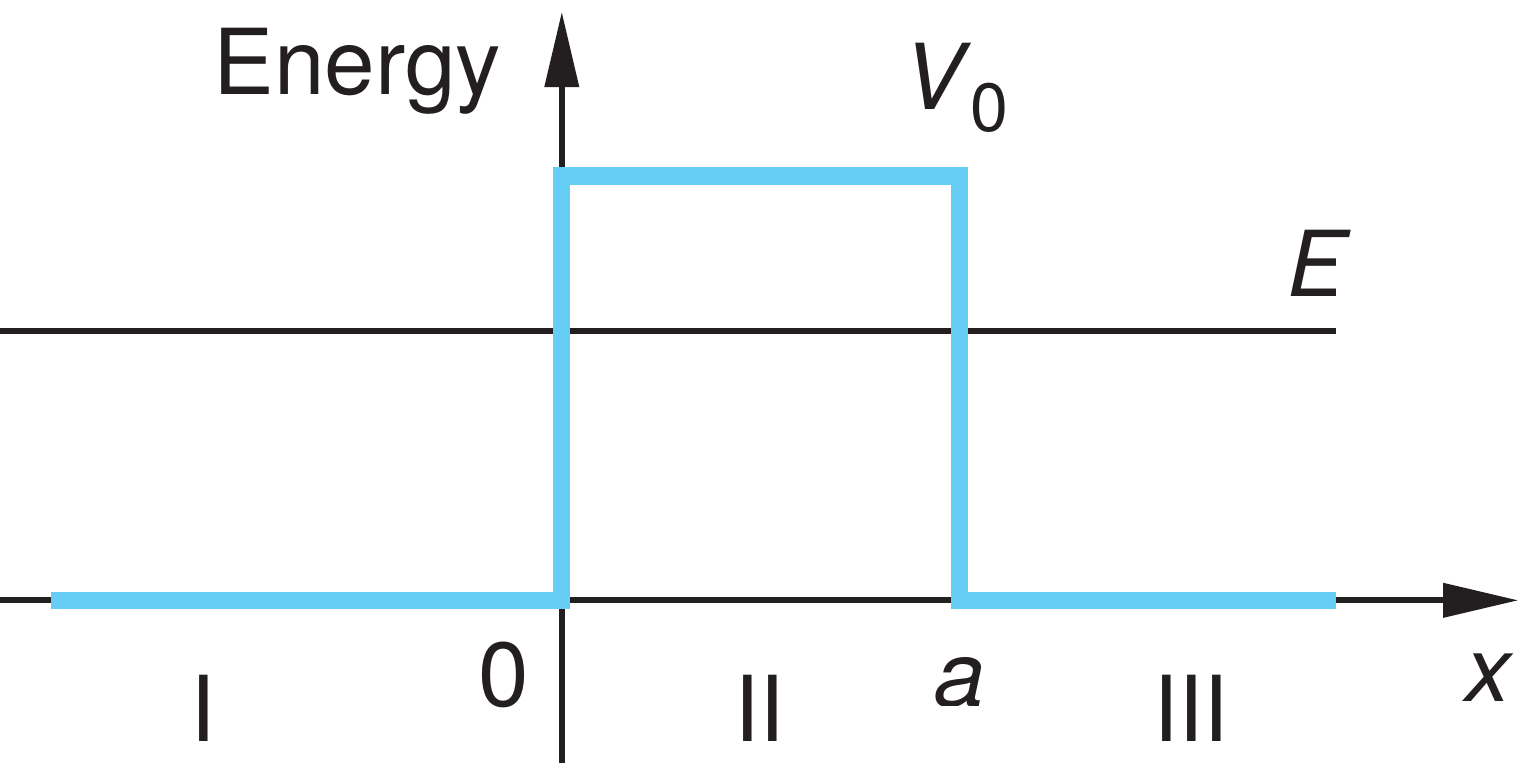
\includegraphics[height=3cm]{figuras/fig33}
          \end{center}
      \end{columns}
    \end{minipage}

\end{frame}

  
%%%%%%%%%%%%%%%%  SLIDE 32 %%%%%%%%%%%%%%%%%%%%%%%%%%

\begin{frame}
  \frametitle{Barreira de Potencial, $E>V_0$}
  
  \fontsize{8pt}{11pt}\selectfont
  
  \vspace*{-1.cm}
    \begin{minipage}[t][20ex][t]{\linewidth}
  
      \begin{columns}
      \column{0.4\linewidth}
          \begin{center}
            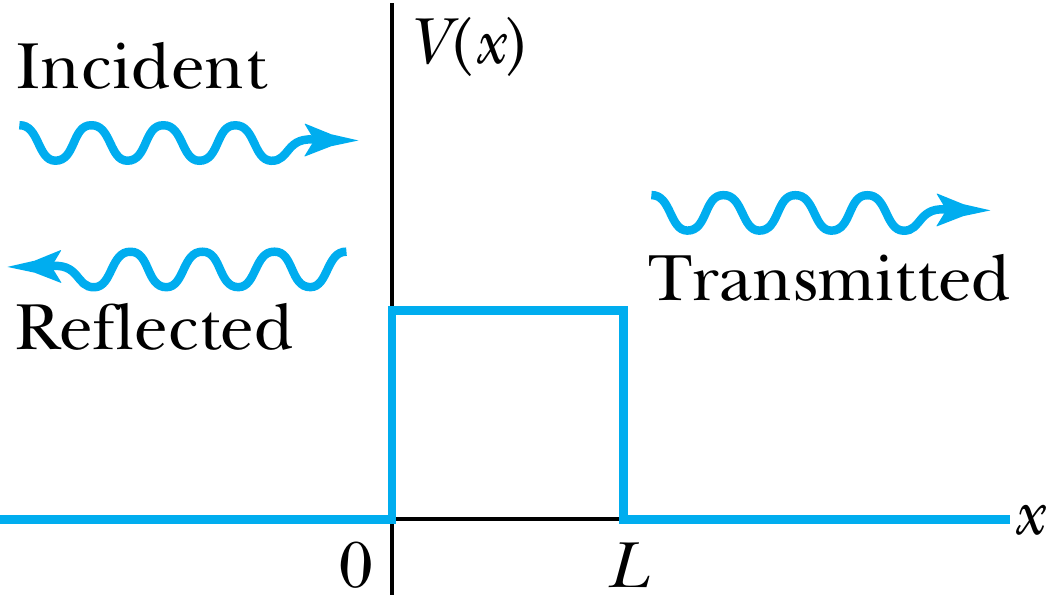
\includegraphics[height=2.5cm]{figuras/fig34}
          \end{center}
        
        \column{0.6\linewidth}
        \[
        \begin{array}[1.2]{lll}
          \text{I} & V=0 & \dfrac{d^2\psi_1}{dx^2}=-\dfrac{2m_pE}{\hbar^2}\psi_1\\
%           &\\
          \text{II} & V=V_0 & \dfrac{d^2\psi_2}{dx^2}=-\dfrac{2m_pE}{\hbar^2}\left(E-V_0\right)\psi_2\\
%           &\\ 
          \text{III} & V=0 & \dfrac{d^2\psi_3}{dx^2}=-\dfrac{2m_pE}{\hbar^2}\psi_3
        \end{array}
          \]
        
        \end{columns}
    \end{minipage}
   
%   
    \begin{minipage}[b][20ex][t]{\linewidth}
  \vspace*{-0.5cm}
      \begin{columns}
        \column{0.5\linewidth}
%         \[
%           \begin{array}[0.8]{lll}
%              \text{Região I}   &  \psi_1(x) = Ae^{ik_1x}+Be^{-ik_1x}\\
%              \text{Região II}  &  \psi_2(x) = Ce^{ik_2x}+De^{-ik_2x}\\
%              \text{Região III} &  \psi_3(x) = Ge^{-ik_1x}\\
%           \end{array}
%         \]

      \[
      \psi(x) = \begin{cases}
                  Ae^{ik_1x}+Be^{-ik_1x}& x < 0\\
                  Ce^{ik_2x}+De^{-ik_2x}& L < x < 0\\
                  Ge^{-ik_1x}& x > L
                \end{cases}
        \]
        onde        
        \begin{align*}
            k_1 &= \sqrt{\dfrac{2m_pE}{\hbar^2}}\\
            k_2 &= \sqrt{\dfrac{2m_p\left( E - V_0 \right)}{\hbar^2}}
          \end{align*}
        
        \column{0.5\linewidth}
        
        O coeficiente de reflexão e Transmissão são dados por
        \[
        \begin{array}[0.8]{lll}
          R &= \dfrac{\left|\, \psi_1 (\text{refletida}) \, \right|^2}{\left|\, \psi_1 (\text{incidente}) \, \right|^2} &= \dfrac{B\cdot B}{A\cdot A}\\
          T &= \dfrac{\left|\, \psi_1 (\text{transmitida}) \, \right|^2}{\left|\, \psi_1 (\text{incidente}) \, \right|^2} &= \dfrac{G\cdot G}{A\cdot A}\\
        \end{array}
        \]
        
        \[
         T_{E>V}= \left[1 + \dfrac{V_0^2\sin^2 \left(k_2\,L \right)}{4E\left(V_0-E\right)}\right]^{-1}
        \]

      
        \end{columns}
    \end{minipage}


\end{frame}

  
%%%%%%%%%%%%%%%%  SLIDE 33 %%%%%%%%%%%%%%%%%%%%%%%%%%

\begin{frame}
  \frametitle{Barreira de Potencial, $E>V_0$}

  \fontsize{8pt}{11pt}\selectfont
  
  \vspace*{-1cm}
  \begin{minipage}[t][20ex][t]{\linewidth}
     $
     \psi(x) =\begin{cases} Ae^{ik_1x}-\dfrac{\beta_L^*}{\alpha_L^*}Ae^{-ik_1x} & x < 0\\
          A\left[ \left( 1-\dfrac{\beta_L^*}{\alpha_L^*} \right)\cos k_2x+ i\dfrac{k_1}{k_2}\left( 1+ \dfrac{\beta_L^*}{\alpha_L^*}\right)\sin k_2x\right] & 0 < x < L\\
          \dfrac{A}{\alpha_L^*}e^{ik_1(x-L)} & x > L
          \end{cases}
    $

  \end{minipage}

  
  \vspace*{-0.5cm}
  \begin{minipage}[b][20ex][t]{\linewidth}
  \begin{columns}
   
    \column{0.4\linewidth}
    
      
    com
     \begin{align*}
            \alpha_L &= \cos k_2L + i\dfrac{k_1^2+k_2^2}{2k_1k_2}\sin k_2L\\
            \beta_L &= -i\dfrac{k_1^2-k_2^2}{2k_1k_2}\sin k_2L
          \end{align*}
    

    
    \column{0.6\linewidth}
    
    \begin{center}
     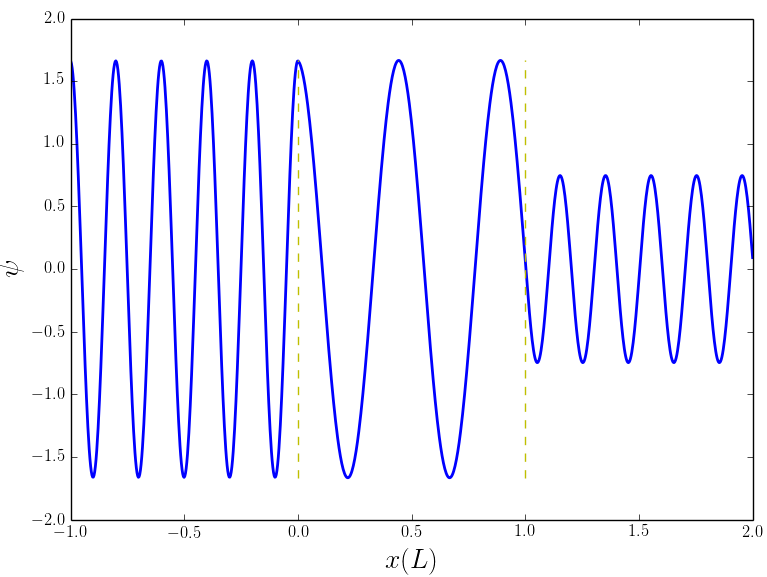
\includegraphics[height=4cm]{figuras/fig35}\\
    \fontsize{8pt}{11pt}\selectfont
    $V_0=0,3eV$, $K=5V_0/4$ e $L=10\,nm$
    \end{center}
   
  \end{columns}
  \end{minipage}

\end{frame}

  
%%%%%%%%%%%%%%%%  SLIDE 33 %%%%%%%%%%%%%%%%%%%%%%%%%%



\begin{frame}
  \frametitle{Barreira de Potencial, $E<V_0$}
  
  \fontsize{8pt}{11pt}\selectfont
  
  \vspace*{-1.cm}
    \begin{minipage}[t][20ex][t]{\linewidth}
  
      \begin{columns}
      \column{0.4\linewidth}
          \begin{center}
            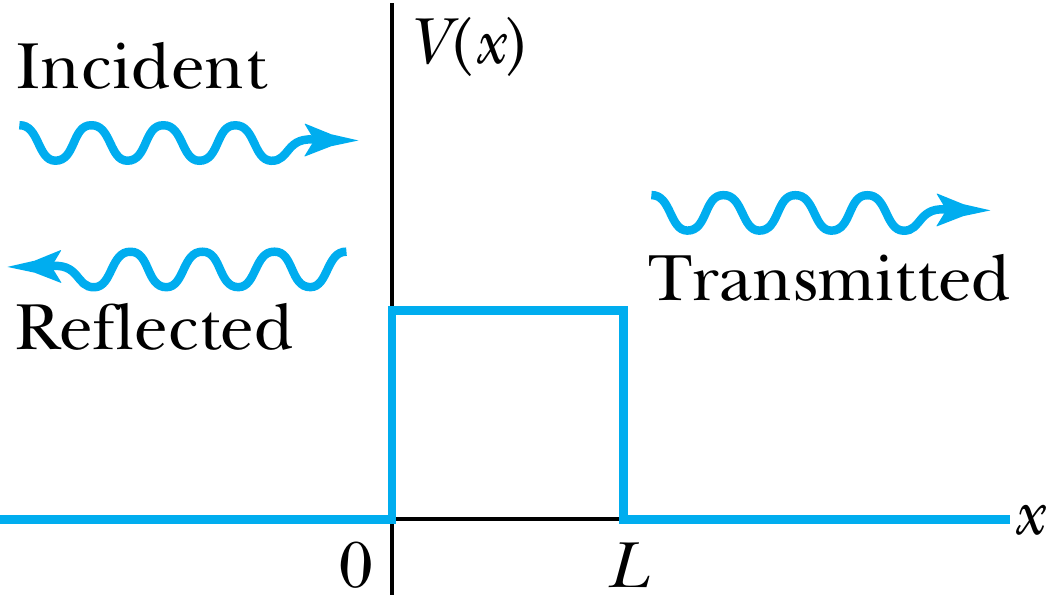
\includegraphics[height=2.5cm]{figuras/fig34}
          \end{center}
        
        \column{0.6\linewidth}
        \[
        \begin{array}[1.2]{lll}
          \text{I} & V=0 & \dfrac{d^2\psi_1}{dx^2}=-\dfrac{2m_pE}{\hbar^2}\psi_1\\
%           &\\
          \text{II} & V=V_0 & \dfrac{d^2\psi_2}{dx^2}=-\dfrac{2m_pE}{\hbar^2}\left(E-V_0\right)\psi_2\\
%           &\\ 
          \text{III} & V=0 & \dfrac{d^2\psi_3}{dx^2}=-\dfrac{2m_pE}{\hbar^2}\psi_3
        \end{array}
          \]
        
        \end{columns}
    \end{minipage}
   
%   
    \begin{minipage}[b][20ex][t]{\linewidth}
  \vspace*{-0.5cm}
      \begin{columns}
        \column{0.5\linewidth}
%         \[
%           \begin{array}[0.8]{lll}
%              \text{Região I}   &  \psi_1(x) = Ae^{ik_1x}+Be^{-ik_1x}\\
%              \text{Região II}  &  \psi_2(x) = Ce^{ik_2x}+De^{-ik_2x}\\
%              \text{Região III} &  \psi_3(x) = Ge^{-ik_1x}\\
%           \end{array}
%         \]

      \[
      \psi(x) = \begin{cases}
                  Ae^{ik_1x}+Be^{-ik_1x}& x < 0\\
                  Ce^{ik_2x}+De^{-ik_2x}& L < x < 0\\
                  Ge^{ik_2x}+He^{-ik_1x}& x > L
                \end{cases}
        \]
        onde        
        \begin{align*}
            k_1 &= \sqrt{\dfrac{2m_pE}{\hbar^2}}\\
            k_2 &= \sqrt{\dfrac{2m_p\left(  V_0 - E \right)}{\hbar^2}}
          \end{align*}
        
        \column{0.5\linewidth}
        
        Os coeficientes de Transmissão é dados por
        
        \[
         T_{E<V}= \left[1 + \dfrac{V_0^2\sinh^2 \left(k_2\,L \right)}{4E\left(V_0-E\right)}\right]^{-1}
        \]

      
        \end{columns}
    \end{minipage}


\end{frame}


  
%%%%%%%%%%%%%%%%  SLIDE 35 %%%%%%%%%%%%%%%%%%%%%%%%%%


\begin{frame}
  \frametitle{Barreira de Potencial, $E>V_0$}

  \fontsize{8pt}{11pt}\selectfont
  
  \vspace*{-1cm}
  \begin{minipage}[t][20ex][t]{\linewidth}
     $
     \psi_{E < V}(x) =\begin{cases} Ae^{ik_1x}-\dfrac{\beta_L^*}{\alpha_L^*}Ae^{-ik_1x} & x < 0\\
          A\left[ \left( 1-\dfrac{\beta_L^*}{\alpha_L^*} \right)\cosh k_2x+ i\dfrac{k_1}{k_2}\left( 1+ \dfrac{\beta_L^*}{\alpha_L^*}\right)\sinh k_2x\right] & 0 < x < L\\
          \dfrac{A}{\alpha_L^*}e^{ik_1(x-L)} & x > L
          \end{cases}
    $

  \end{minipage}

  
  \vspace*{-0.5cm}
  \begin{minipage}[b][20ex][t]{\linewidth}
  \begin{columns}
   
    \column{0.4\linewidth}
    
      
    com
     \begin{align*}
            \alpha_L &= \cosh k_2L + i\dfrac{k_1^2-k_2^2}{2k_1k_2}\sinh k_2L\\
            \beta_L &= -i\dfrac{k_1^2+k_2^2}{2k_1k_2}\sinh k_2L
          \end{align*}
    

    
    \column{0.6\linewidth}
    
    \begin{center}
     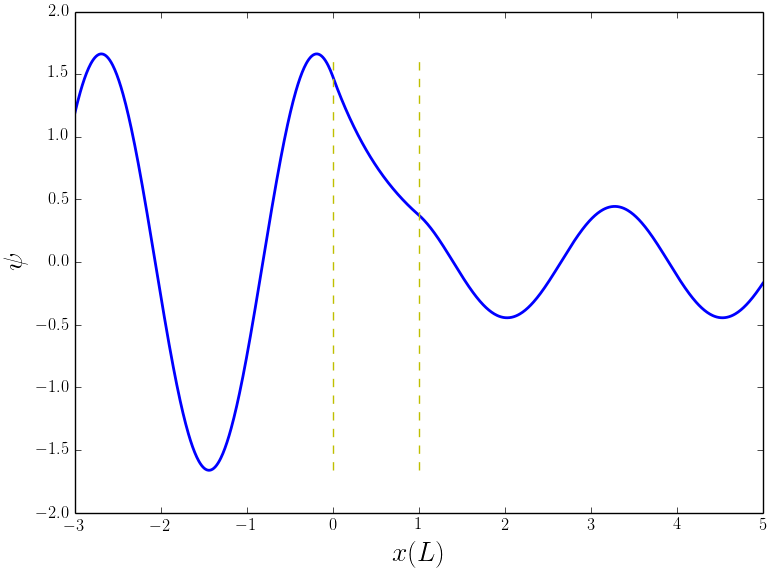
\includegraphics[height=4cm]{figuras/fig36}\\
    \fontsize{8pt}{11pt}\selectfont
    $V_0=0,3eV$, $K=8V_0/10$ e $L=10\,nm$
    \end{center}
   
  \end{columns}
  \end{minipage}

\end{frame}



  
%%%%%%%%%%%%%%%%  SLIDE 35 %%%%%%%%%%%%%%%%%%%%%%%%%%


\begin{frame}
  \frametitle{Aplicação - Microscópio de Tunelamento}
  \fontsize{9pt}{11pt}\selectfont
  
  \begin{columns}
   
    \column{0.4\linewidth}
    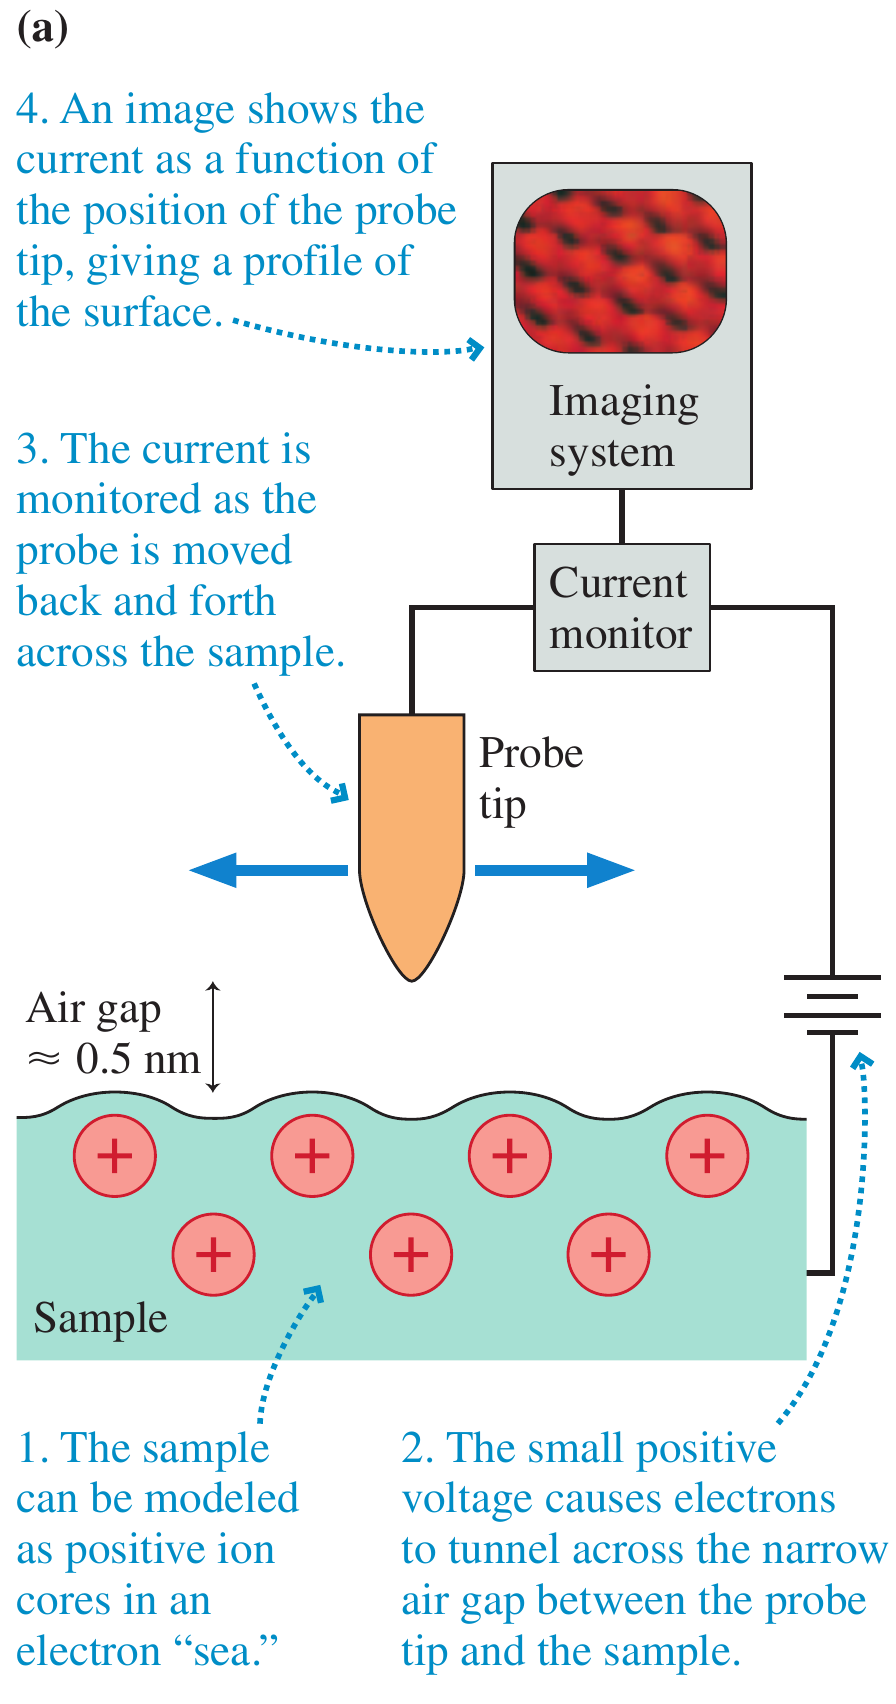
\includegraphics[height=8cm]{figuras/fig37}
    \column{0.6\linewidth}
    \begin{center}
     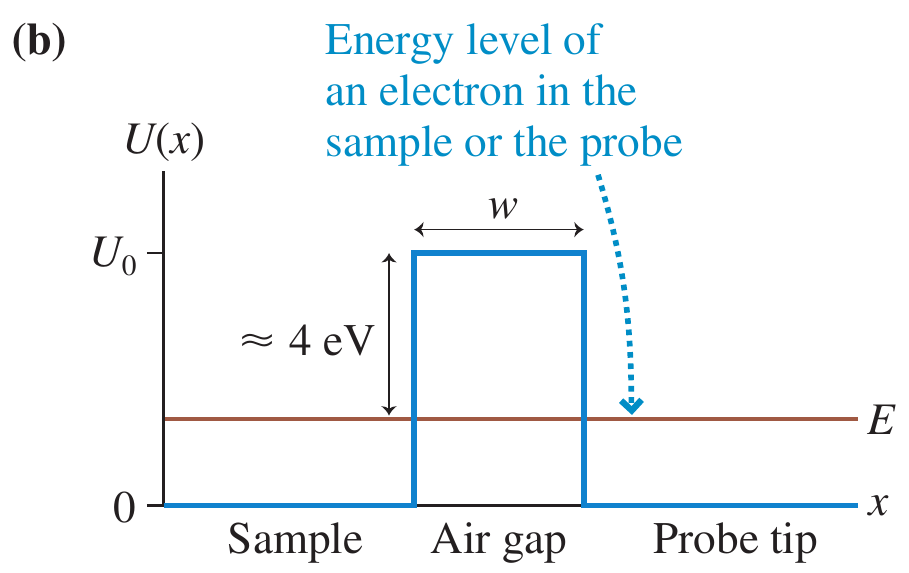
\includegraphics[width=5cm]{figuras/fig37b}
    \end{center}
    \vspace*{0.5cm}
    Em essência consiste de um efeito fotoelétrico no qual a função trabalho é $\Phi\approx 4 eV$.  O fóton que é emitido pela ponta na direção da superfície tem energia menor do que $4 eV$, mas como a largura da barreira (de ar) é fina, os elétrons podem tunelar em direção à ponta.
  \end{columns}

\end{frame}


  
%%%%%%%%%%%%%%%%  SLIDE 37 %%%%%%%%%%%%%%%%%%%%%%%%%%


\begin{frame}
  \frametitle{Aplicação - Decaimento alfa}
  \fontsize{9pt}{11pt}\selectfont
  
  \begin{center}
   \animategraphics[autoplay,loop,width=5.5cm]{10}{alfa/alfa-}{0}{24}
  \end{center}
  
  \begin{columns}
  
    \column{0.5\linewidth}
    
    Uma das aplicações mais impressionantes é a dada por Gamow para explicar o decaimento $\alpha$ dos átomos. O processo consiste no decaimento de núcleos pesados em núcleos menos pesados via a emissão de partículas $\alpha$, átomos de $He^4$. Usando uma notação compacta podemos escrever 
    \[
     \,^Z_NX^A \longrightarrow \,^{(Z-2)}_{(N-2)}X^{(A-4)}+\,^2_2He^4
    \]
    
    \column{0.5\linewidth}
    
    onde $Z$, $N$, e $A$ são, respectivamente, o número de prótons, nêutrons e o total de nucleões na especie nuclear denotada por $X$ (o núcleo pai) ou $Y$ (o núcleo filho).\\
    
    Tipicamente o valor das grandezas envolvidas no decaimento $\alpha$ estão dadas por
    \begin{align*}
     R \sim 2-4\,F, & E_\alpha \sim 2-8\,MeV,\\
     Z \sim 50-100 &
    \end{align*}
    
  \end{columns}

\end{frame}


  
%%%%%%%%%%%%%%%%  SLIDE 37 %%%%%%%%%%%%%%%%%%%%%%%%%%


\begin{frame}
  \frametitle{Átomo de Hidrogênio}
  \fontsize{9pt}{11pt}\selectfont
  
  Como sabemos o átomo de hidrogênio consiste de um eletron sujeito ao potencial $V$ gerado pelo próton do núcleo, dado por
        \[
          V = - \dfrac{q^2}{r}\;\;\;\;\; q^2=\dfrac{e^2}{4\pi\epsilon_0}
          \nonumber
        \]
  dessa forma a equação de Schrödinger para o elétron fica escrita como
  \[
   \left[ -\dfrac{\hbar}{2} \left( \dfrac{1}{m_e}+\dfrac{1}{m_p} \right)\Delta_r-\dfrac{\hbar}{2} \dfrac{1}{m_e+m_p}\Delta_\xi -  \dfrac{q^2}{r}\right] \Phi\left(r,\,\xi,\,t \right) = i\hbar \dfrac{\partial \Phi\left(r,\,\xi,\,t \right)}{\partial t}
  \]
  onde $r$ é a distância entre o elétron e o próton e $\xi$ é a posição do centro de massas e $\mu$ é a massa reduzida. Utilizando separação de variáveis
  \[
   \Phi\left(r,\,\xi,\,t \right) = \Psi(r,\,t)\mathcal{X}(\xi,\,t)
  \]

  de onde
  \[
  \begin{cases}
   \left( -\dfrac{\hbar}{2\mu}\Delta_r - \dfrac{q^2}{r}\right)  \Psi\left(r,\,t \right) &= i\hbar \dfrac{\partial \Psi\left(r,\,t \right)}{\partial t}\\
   \dfrac{\hbar}{2M} \Delta_\xi \, \mathcal{X}\left(\xi,\,t \right) &= i\hbar  \dfrac{\partial \mathcal{X}\left(\xi,\,t \right)}{\partial t}
  \end{cases}
\]

\end{frame}


  
%%%%%%%%%%%%%%%%  SLIDE 39 %%%%%%%%%%%%%%%%%%%%%%%%%%


\begin{frame}
  \frametitle{Átomo de Hidrogênio}
  \fontsize{9pt}{11pt}\selectfont
  
  
  
  \vspace*{-1cm}
  \begin{minipage}[t][20ex][t]{\linewidth}
  
  \begin{columns}
          \column{0.5\linewidth}
          Agora vamos separar a parte temporal da espacial da equação para o elétron (já que V não depende do tempo) utilizando 

        \[
          \Psi = \psi(x)e^{-i\frac{E}{\hbar}t}
        \]
        de onde
        \[
          \Delta \psi + \dfrac{2m}{\hbar^2}\left( E + \dfrac{q^2}{r} \right)\psi = 0
        \]
        Dada a simetria do problema é adequado trabalhar no sistema de coordenadas esféricas:
        
        \column{0.5\linewidth}
        
        
        
        \[
          \begin{align*}
            x &= r\cos \theta \sin \phi\\
            y &= r\cos \theta \cos \phi\\
            z &= r\sin\theta
          \end{align*}
        \]
        \begin{center}
        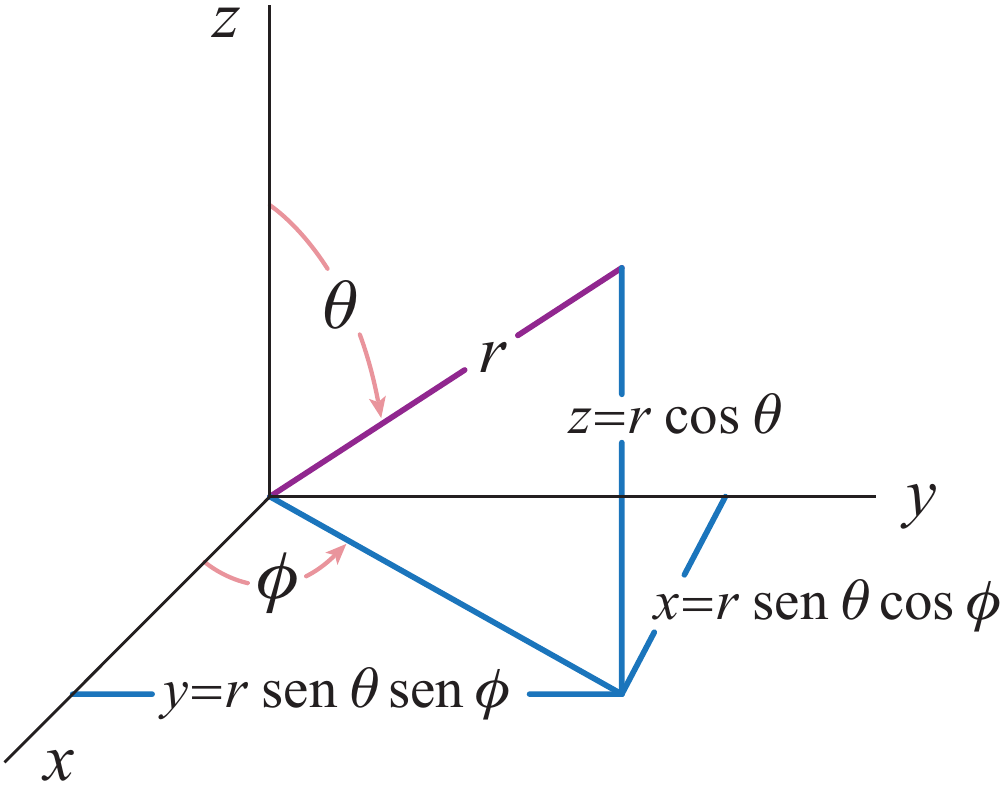
\includegraphics[width=4.5  cm]{figuras/fig38}
        \end{center}
        \end{columns}
   
  \end{minipage}

  
  \vspace*{0.5cm}
  \begin{minipage}[t][20ex][b]{\linewidth}
  O que resulta em
          \[
          \left[ \dfrac{1}{r^2} \dfrac{\partial \,}{\partial r}\left(r^2\dfrac{\partial\,}{\partial r} \right) + \dfrac{1}{r^2\sin^2\theta}\dfrac{\partial^2 \,}{\partial \phi^2}+ \dfrac{1}{r^2\sin \theta }\dfrac{\partial \,}{\partial \theta}\left(\sin \theta\dfrac{\partial \,}{\partial \theta} \right) \right]\psi + \dfrac{2m}{\hbar^2}\left( E + \dfrac{q^2}{r} \right)\psi = 0
        \]  
  \end{minipage}
  
\end{frame}


  
%%%%%%%%%%%%%%%%  SLIDE 40 %%%%%%%%%%%%%%%%%%%%%%%%%%


\begin{frame}
  \frametitle{Átomo de Hidrogênio - Sol. Angular}
  \fontsize{8pt}{11pt}\selectfont
  
  
  \begin{columns}[T]
    
    \column{0.45\linewidth}
    
      Propomos uma primeira separação de variáveis\vspace{-0.5cm}
    
      \[
        \psi\left( r,\,\theta,\,\phi\right) = R(r)Y(\theta,\,\phi)
      \]
      
      que resulta em uma equação só com a parte radial
      \[
      \dfrac{d\,}{dr}r^2\dfrac{d\,}{dr} +\dfrac{2mr^2}{\hbar^2}\left( E + \dfrac{q^2}{r} \right) = \lambda R
      \]
      
      e outra só com a parte angular ($\theta$ ângulo polar e $\phi$ ângulo azimutal)\vspace{-0.5cm}
      
      \[
        \dfrac{1}{\sin^2\theta}\dfrac{d^2 Y}{d \phi^2}+ \dfrac{1}{\sin \theta }\dfrac{d Y}{d \theta}\left(\sin \theta\dfrac{d Y}{d \theta} \right) = -\lambda Y
      \]
      
      Para esta equação propomos uma nova separação de variáveis

      \[
      Y(\theta,\, \phi) = \Theta(\theta) \Phi(\phi)
      \]
      
      que resulta em
      
    \column{0.02\linewidth}
        \rule{.1mm}{0.7\textheight}
    
    \column{0.53\linewidth}
      \vspace{-0.5cm}
      
      \[
      \dfrac{1}{\Theta}\left[\sin \theta\dfrac{d \Theta}{d \theta}\left(\sin \theta\dfrac{d Y}{d \theta} \right) + \lambda \Theta\sin^2 \theta \right] =  - \dfrac{1}{\Phi}\dfrac{d^2 \Phi}{d \phi^2}
      \]


      que nos leva a duas outras EDOs, uma para parte polar\vspace{-0.3cm}
      
      \[
      \sin \theta\dfrac{d \Theta}{d \theta}\left(\sin \theta\dfrac{d Y}{d \theta} \right) + \lambda \Theta\sin^2 \theta = m^2\Theta
      \]
      
      e para parte azimutal
      \[
        \dfrac{d^2 \Phi}{d \phi^2} = -m^2\Phi
      \]
      
      que tem por solução
      
      \[
       \Phi(\phi) = \dfrac{1}{\sqrt{2\pi}}\exp\left(im\phi\right)
      \]
      
      onde
      \[
       m\in\mathbb{Z}=0,\,\pm 1,\, \pm 2,\,\ldots
      \]
      
      é conhecida como número quântico magnético.     
  \end{columns}
\end{frame}



  
%%%%%%%%%%%%%%%%  SLIDE 41 %%%%%%%%%%%%%%%%%%%%%%%%%%


\begin{frame}
  \frametitle{Átomo de Hidrogênio - Sol. Angular}
  \fontsize{7pt}{11pt}\selectfont
  
  
  \begin{columns}[T]
  
  
    \column{0.49\linewidth}
    Para solucionar a EDO paras a parte polar devemos aplicar a substitução de variáveis $w=\cos \theta$ o que explicita a equação como sendo a EDO associada de Legendre 
    \[
     \dfrac{d}{dw}\left( (1-w^{2})\dfrac{dP}{dw} \right) + \left[ \lambda^2 - \dfrac{m^{2}}{1-w^{2}} \right]P = 0
    \]
    que é a equação diferencial da função associada de Legendre, a qual, utilizando a relação de Rodriguez
    \[
     P_l^m(w)=(-1)^m(1-w^2)^{\frac{m}{2}} \dfrac{\mathrm d^m P_l}{\mathrm d w^m}
    \]
    
    nos leva à equação de Legendre, que tem por solução
    \[
     P_l(w)=\left(a_0\sum_{k=0}^{\infty}\frac{a_{2k}}{a_0}w^{2k}+a_1\sum_{k=1}^{\infty}\frac{a_{2k+1}}{a_1}w^{2k+1}\right)
    \]

    
    
    \column{0.02\linewidth}
        \rule{.1mm}{0.7\textheight}
    
    \column{0.49\linewidth}
    

    onde a relação de recorrência\vspace*{-0.25cm}
    
    \[
     \dfrac{a_{k+2}}{a_k} = \dfrac{(k+m)(k+m+1)-\lambda ^2}{(k+1)(k+2)}
    \]

    nos leva a concluir que a série não converge o que força a estabelecer um corte exigindo que $(k+m)(k+m+1)-\lambda^2 = 0$, e se definimos $l \equiv k + m$, resulta em\vspace*{-0.25cm}
    \[
     \lambda = l(l+1)\vspace*{-0.25cm}
    \]
    Com esto, $P_l$ resulta em um polinômio de ordem $l$ já que $k=l-m$, isso exige que como $k \geq 0$, então $m \leq l$. Como na relação de Rodriguez tratamos com derivadas então $m$ deve ser positivos, então\vspace*{-0.25cm}
    \[
     \left|\, m \,\right|  \leq l \Rightarrow  -l \leq  m  \leq l\vspace*{-0.25cm}
    \]
    de forma que $m$ pode assumir os valore $-l$, $-l+1$, $\ldots$, $-1$, $0$, $1$, $\ldots$, $l-1$, $l$  

   
  \end{columns}
\end{frame}


  
%%%%%%%%%%%%%%%%  SLIDE 42 %%%%%%%%%%%%%%%%%%%%%%%%%%


\begin{frame}
  \frametitle{Átomo de Hidrogênio - Sol. Angular}
  \fontsize{7pt}{11pt}\selectfont
  
  
  \begin{columns}[T]

    \column{0.49\linewidth}
    
    Reunindo os resultado anteriores e calculando a condição de normalização obtemos
    
    \[
     Y_{lm}\left( \theta,\phi \right) = \sqrt{\dfrac{2(l+\left| \,  m \, \right|)!}{(l-{\left| \, m  \, \right|})!(2l+1)}}\; P_l^m(\cos \theta)\exp \left( im\phi \right)
    \]
    Estas funções são chamadas de harmônicos esféricos; são funções ortonormalizadas de forma que podem expressar estados diferentes da função de onda
    
    \begin{center}
      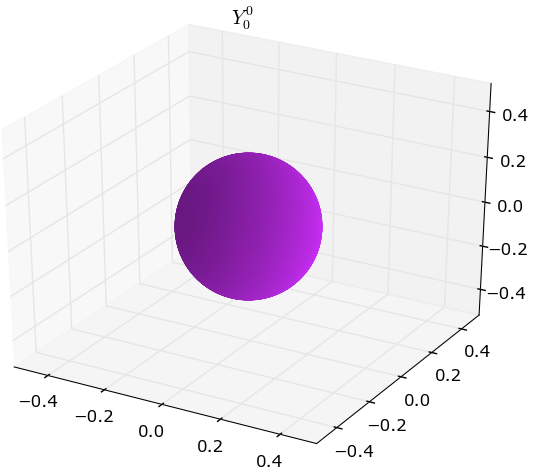
\includegraphics[height=2.5cm]{figuras/fig39}\\
      \fontsize{8pt}{11pt}\selectfont
      $Y_{0,0}(\theta, \phi) = \frac{1}{2 \sqrt{\pi}}$
    \end{center}
    
    
%     \column{0.02\linewidth}
%         \rule{.1mm}{0.7\textheight}
    
    \column{0.49\linewidth}
    
    \begin{center}
      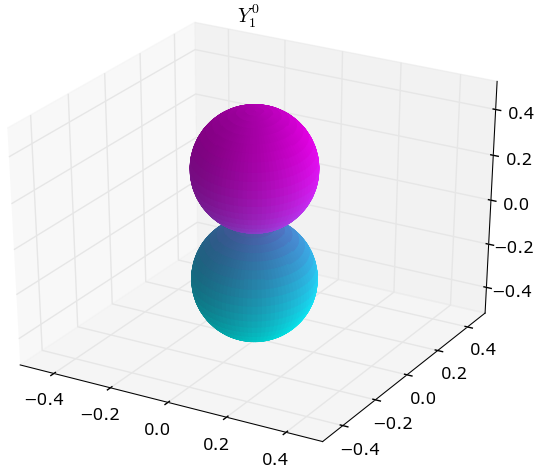
\includegraphics[height=2.5cm]{figuras/fig40}\\
      \fontsize{8pt}{11pt}\selectfont
      $Y_{1,0}(\theta, \phi) = \frac{\sqrt{3}}{2\sqrt{\pi}} \cos \theta$
    \end{center}
    
    
    \begin{center}
      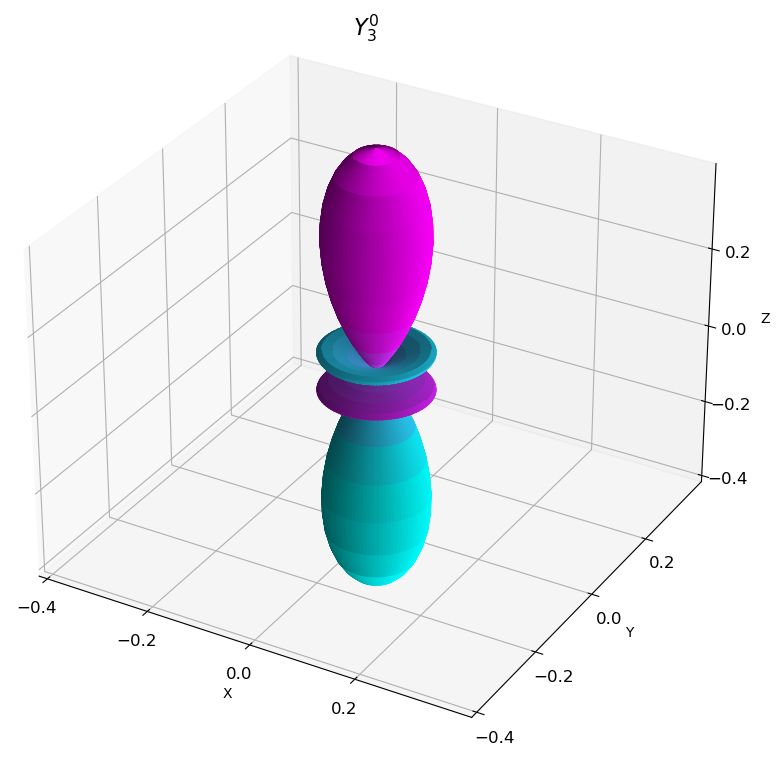
\includegraphics[height=2.75cm]{figuras/fig41}\\
      \fontsize{8pt}{11pt}\selectfont
      $Y_{3,0}(\theta, \phi) = \frac{\sqrt{7} \left(5 \cos^{2}{\left(\theta \right)} - 3\right) \cos{\left(\theta \right)}}{4 \sqrt{\pi}}$

    \end{center}
    
  \end{columns}
   
\end{frame}



%%%%%%%%%%%%%%%%  SLIDE 44 %%%%%%%%%%%%%%%%%%%%%%%%%%


\begin{frame} 
  \frametitle{Átomo de Hidrogênio - Sol. Radial}
  \fontsize{8pt}{11pt}\selectfont
  
  A EDP de Schrödinger para o átomo de hidrogênio em coordenadas esféricas é
  
  \begin{align*}
    \left[ \dfrac{1}{r^2} \dfrac{\partial \,}{\partial r}\left(r^2\dfrac{\partial\,}{\partial r} \right) + \dfrac{1}{r^2\sin^2\theta}\dfrac{\partial^2 \,}{\partial \phi^2}+ \dfrac{1}{r^2\sin \theta }\dfrac{\partial \,}{\partial \theta}\left(\sin \theta\dfrac{\partial \,}{\partial \theta} \right) \right]R(r)Y(\theta,\,\phi)\qquad&\\
    + \dfrac{2m}{\hbar^2}\left( E + \dfrac{q^2}{r} \right)R(r)Y(\theta,\,\phi) &=0\\
    Y(\theta,\,\phi)\left[ \dfrac{1}{r^2} \dfrac{\partial \,}{\partial r}\left(r^2\dfrac{\partial\,}{\partial r} \right)\right]R(r) +  L^2 R(r)Y(\theta,\,\phi)+ Y(\theta,\,\phi)\dfrac{2m}{\hbar^2}\left( E + \dfrac{q^2}{r} \right)R(r) &= 0\\
    Y(\theta,\,\phi)\left[ \dfrac{1}{r^2} \dfrac{\partial \,}{\partial r}\left(r^2\dfrac{\partial\,}{\partial r} \right)\right]R(r) - \left[  \dfrac{l(l+1)}{r^2} \right]Y(\theta,\,\phi)R(r)+ Y(\theta,\,\phi)\dfrac{2m}{\hbar^2}\left( E + \dfrac{q^2}{r} \right)R(r) &= 0\\
            -\dfrac{\hbar^2}{2m}\left[\dfrac{1}{r^2} \dfrac{\partial \,}{\partial r}\left(r^2\dfrac{\partial\,}{\partial r} \right)\right]R(r) + \left[ \dfrac{\hbar^2}{2m} \dfrac{l(l+1)}{r^2} - \dfrac{q^2}{r} \right]R(r) &= E\,R(r)
  \end{align*}
  
  se supomos que, $u(r) \equiv r\,R$, e substituirmos na EDP, chegamos
  
  \[
   -\dfrac{\hbar^2}{2m}\dfrac{d^2u}{d r^2} + \left[ \dfrac{\hbar^2}{2m} \dfrac{l(l+1)}{r^2} - \dfrac{q^2}{r} \right]u = E\,u
  \]
  
  que é nossa EDO radial
  
\end{frame}


%%%%%%%%%%%%%%%%  SLIDE 45 %%%%%%%%%%%%%%%%%%%%%%%%%%


\begin{frame} 
  \frametitle{Átomo de Hidrogênio - Sol. Radial}
  \fontsize{8pt}{11pt}\selectfont
  
  
    \begin{columns}[T]

      \column{0.45\linewidth}
      
        Admitamos que
        \[
        V_{\text{ef}} \equiv \dfrac{\hbar^2}{2m}\dfrac{l(l+1)}{r^2} - \dfrac{q^2}{r}
        \]
        onde
        
        \begin{align*}
          \dfrac{\hbar^2}{2m} &= 6,104263784201592\times^{-39}J\,m^2\\
          \dfrac{q^2}{r} &= 2,307077352370616\times 10^{-28} J\,m
        \end{align*}
      
      
      \column{0.55\linewidth}
      
%       \vspace*{-0.5cm}
      \begin{center}
        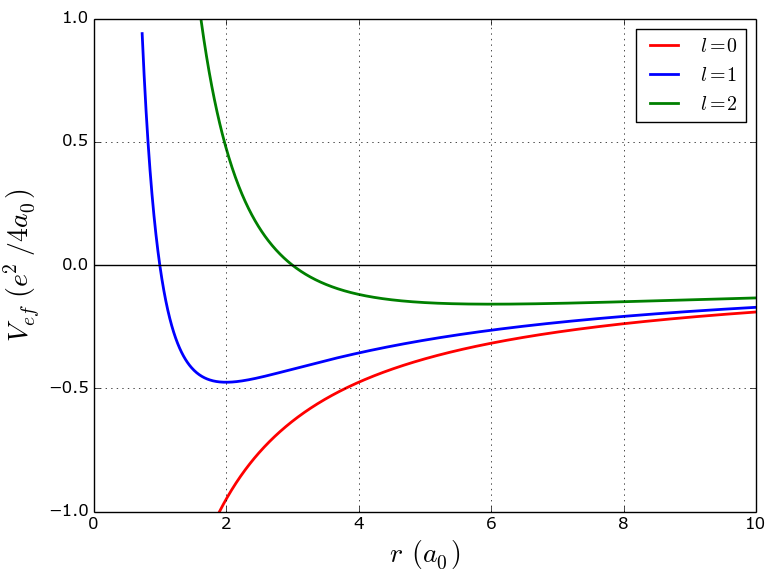
\includegraphics[height=5cm]{figuras/fig42}
      \end{center}
    
    \end{columns}
  
    
    
    Analisando o comportamento assintótico como sol. a EDO radial obtemos
    \[
     u_{r \to \infty} = A_2e^{\lambda r} + B_2 e^{-\lambda r}
    \]
    onde
    \[
     \lambda = \dfrac{\sqrt{2mE}}{\hbar}
    \]


\end{frame}


%%%%%%%%%%%%%%%%  SLIDE 46 %%%%%%%%%%%%%%%%%%%%%%%%%%


\begin{frame} 
  \frametitle{Átomo de Hidrogênio - Sol. Radial}
  \fontsize{8pt}{11pt}\selectfont
  
    
    \begin{columns}[T]

      \column{0.5\linewidth}
    Como solução geral para a EDO radial propomos uma solução por séries finita ($N$ termos)
    \vspace*{-0.5cm}
    \[
     u(r) = r^{l+1}e^{-\lambda r}\sum_{k=0}^N A_kr^k\vspace*{-0.4cm}
    \]
    e para facilitar os cálculos propõe-se a mudança de variável\vspace*{-0.4cm}
    \[
     u(r) = r^{l+1}f(r)e^{-\lambda r}\vspace*{-0.4cm}
    \]
    
    que altera a EDO para\vspace*{-0.2cm}
    
    \[
    \begin{align*}
      \dfrac{d^2f}{dr^2} + 2\left[ \dfrac{\left(l+1 \right)}{r} - \lambda \right]\dfrac{df}{dr}\qquad\qquad &\\
        + \dfrac{2}{r}\left[ -\lambda\left( l+1 \right) + \dfrac{q^2m}{\hbar^2}\right]f = 0       & 
    \end{align*}\vspace*{-0.3cm}
    \]
    
    onde usamos que $E = -\dfrac{\hbar^2}{2m}\lambda^2$. A série solução resulta na relação de recorrência
    \vspace*{-0.4cm}
    \[
     \dfrac{A_{k}}{A_{k-1}} = 2\left[ \dfrac{\lambda\left( k+l \right) - \dfrac{q^2m}{\hbar^2}}{k\left(k+2l+1 \right)} \right]\vspace*{-0.4cm}
    \]
    
    \column{0.5\linewidth}
    
    Como a série deve ser zero desde o termo $N+1$
    \vspace*{-0.5cm}
    \[
    \begin{align*}
      \lambda\left( N+1+l \right) - \dfrac{q^2m}{\hbar^2} &=0\\
      \lambda &= \dfrac{q^2m}{\hbar^2\left( N+1+l \right)}\\
      \dfrac{\sqrt{2mE}}{\hbar} &= - \dfrac{q^2m}{\hbar^2\left( k+l \right)}\\
            E&= - \dfrac{q^4m}{2\hbar^2\left( N+1+l \right)}\vspace*{-0.4cm}
    \end{align*}\vspace*{-0.3cm}
    \]
    
    Se $n=N=l+1$,e então\vspace*{-0.2cm}
    \[
     E_n = - \dfrac{q^4m^2}{2n^2\hbar^4} = - \left(\dfrac{q^2}{2a_0}\right)\dfrac{1}{n^2}
     \vspace*{-0.2cm}
    \]
    onde $n$ é o número quântico principal e $N$ o número quântico radial.  Como $N$ é um número inteiro e $l$ é o número quântico do momento angular
    \[
     l \leq n-1
    \]
    
    \end{columns}
          
  \end{frame}
  
  

%%%%%%%%%%%%%%%%  SLIDE 46 %%%%%%%%%%%%%%%%%%%%%%%%%%


\begin{frame} 
  \frametitle{Átomo de Hidrogênio - Sol. Radial}
  \fontsize{8pt}{11pt}\selectfont
  
    
%     \begin{columns}[T]
%     
%     \column{0.5\linewidth}
%     
%     
% 
%     
%     \column{0.5\linewidth}
%     
%     
%     
%     \end{columns}
    
    Substituindo os resultados obtidos na EDO original
    
    \[
     \dfrac{d^2f}{dr^2} + 2\left[ \dfrac{\left(l+1 \right)}{r} - \lambda \right]\dfrac{df}{dr} + \dfrac{2}{r}\left[ -\lambda\left( l+1 \right) + n\lambda\right]f = 0
    \]
    mudando de variável $\rho = 2\lambda\,r$, resulta em
    \[
     \rho \dfrac{d^2g}{d\rho^2} + \left[ \left(2l+1 \right) + 1 - \rho \right]\dfrac{dg}{d\rho} + \left[ \left( n + l \right) - \left( 2l + l \right)  \right]g = 0
    \]
    
    Que é a EDO de Laguere com solução dada por
    \[
     L_q^p(x) = \sum_{k = 0}^{q - p}\dfrac{(-1)^k\left( q! \right)^2x^k}{\left( p - q - k\right)!\left( p+k \right)!k!}
    \]
        sendo assim, podemos retornar a nossas variáveis originais e aplicada as condições de normalização, o qual resulta
    \[
     R_{nl} = -\left(\dfrac{2}{na_0}\right)^{3/2}\sqrt{\dfrac{2n\left[ \left(  n+l\right) \right]^3}{\left( n-l-1 \right)!}}\left( \dfrac{2r}{na_0} \right)^l\exp \left( -\dfrac{r}{na_0} \right)L_{n+l}^{2l+1}\left(\dfrac{2r}{na_0}\right)
    \]
          
  \end{frame}
  
  

%%%%%%%%%%%%%%%%  SLIDE 46 %%%%%%%%%%%%%%%%%%%%%%%%%%


\begin{frame} 
  \frametitle{Átomo de Hidrogênio - Sol. Radial}
  \fontsize{8pt}{11pt}\selectfont
  
  \vspace*{-1cm}
    
    \begin{columns}[T]
    
    \column{0.55\linewidth}
    
    \begin{align*}
            R_{1,0} &=  2 a_0^{-3/2}e^{- \frac{r}{a_0}} \\
            R_{2,0} &=  \frac{\sqrt{2}}{4a_0^{3/2}} \left(2 - \frac{r}{a_0}\right) e^{- \frac{r}{2a_0}} \\
            R_{2,1} &=  \frac{\sqrt{6} r}{12a_0^{5/2}} e^{- \frac{r}{2a_0}} \\
            R_{3,0} &=  \frac{2 \sqrt{3}}{27a_0^{3/2}} \left(\frac{2 r^{2}}{9a_0^2} - \frac{2r}{a_0} + 3\right) e^{- \frac{r}{3a_0}} \\
            R_{3,1} &=  \frac{\sqrt{6} r}{81a_0^{3/2}} \left(- \frac{2 r}{3a_0^2} + 4\right) e^{- \frac{r}{3a_0}} \\
            R_{3,2} &=  \frac{2 \sqrt{30}}{1215} \frac{r^2}{a_0^{7/2}} e^{- \frac{r}{3a_0}} \\
            R_{4,0} &=  a_0^{-3/2}\left(- \frac{r^{3}}{768a_0^3} + \frac{r^{2}}{32a_0^2} - \frac{3 r}{16a} + \frac{1}{4}\right) e^{- \frac{r}{4a_0}} 
          \end{align*}

    
    \column{0.45\linewidth}
    
    
    
    \begin{center}
     \hspace*{-2cm} 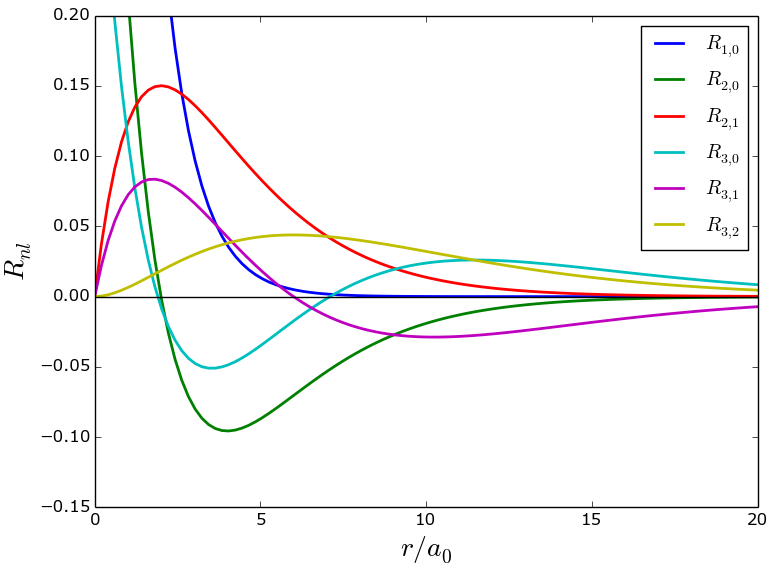
\includegraphics[height=5cm]{figuras/fig43}
    \end{center}
    
    \end{columns}
          
  \end{frame}
  
%%%%%%%%%%%%%%%%  SLIDE 46 %%%%%%%%%%%%%%%%%%%%%%%%%%


\begin{frame} 
  \frametitle{Átomo de Hidrogênio - Resumo}
  \fontsize{9pt}{11pt}\selectfont
  
    Finalmente, a função de onda total é dada por
    \[
     \psi_{nlm_l}(r,\theta,\phi) = R_{nl}Y_{lm_l}(\theta,\phi)
    \]
    
    \begin{itemize}
      \item A energia de qualquer nível é dada por
      \[
        E_n = - \left(\dfrac{q^2}{2a_0}\right)\dfrac{1}{n^2},\qquad a_0 = \dfrac{4\pi\epsilon_0\,\hbar^2}{m\,e^2} =\dfrac{\hbar^2}{q^2m}
      \]

     \item Os níveis de energia são \textbf{degenerados} em relação a $l$, e cada um desse nível subníveis ou subcamadas, como também chamados, historicamente recebem a seguinte notação
     \begin{center}
        \begin{tblr}{
        hlines = {1pt, blue},
        vlines = {1pt, blue},
%         colspec={XXXXXXXXX},
  %       colspec={X[-1,c,0.05\textwidth]X[1,c,0.2\textwidth]X[1,c,0.2\textwidth]},
  %       row{1} = {cabezeraTabela,fg=black},
        column{1} = {blue!10},
        }
        $l$ & 0 & 1 & 2 & 3 & 4 & 5 & 6 &\ldots \\
        notação & s & p & d & f & g & h & i & \ldots \\
      \end{tblr}      
    \end{center}
     
    \end{itemize}
    
  \end{frame}


  
%%%%%%%%%%%%%%%%  SLIDE 49 %%%%%%%%%%%%%%%%%%%%%%%%%%


\begin{frame} 
  \frametitle{Átomo de Hidrogênio - Resumo}
  
  
      \begin{center}
        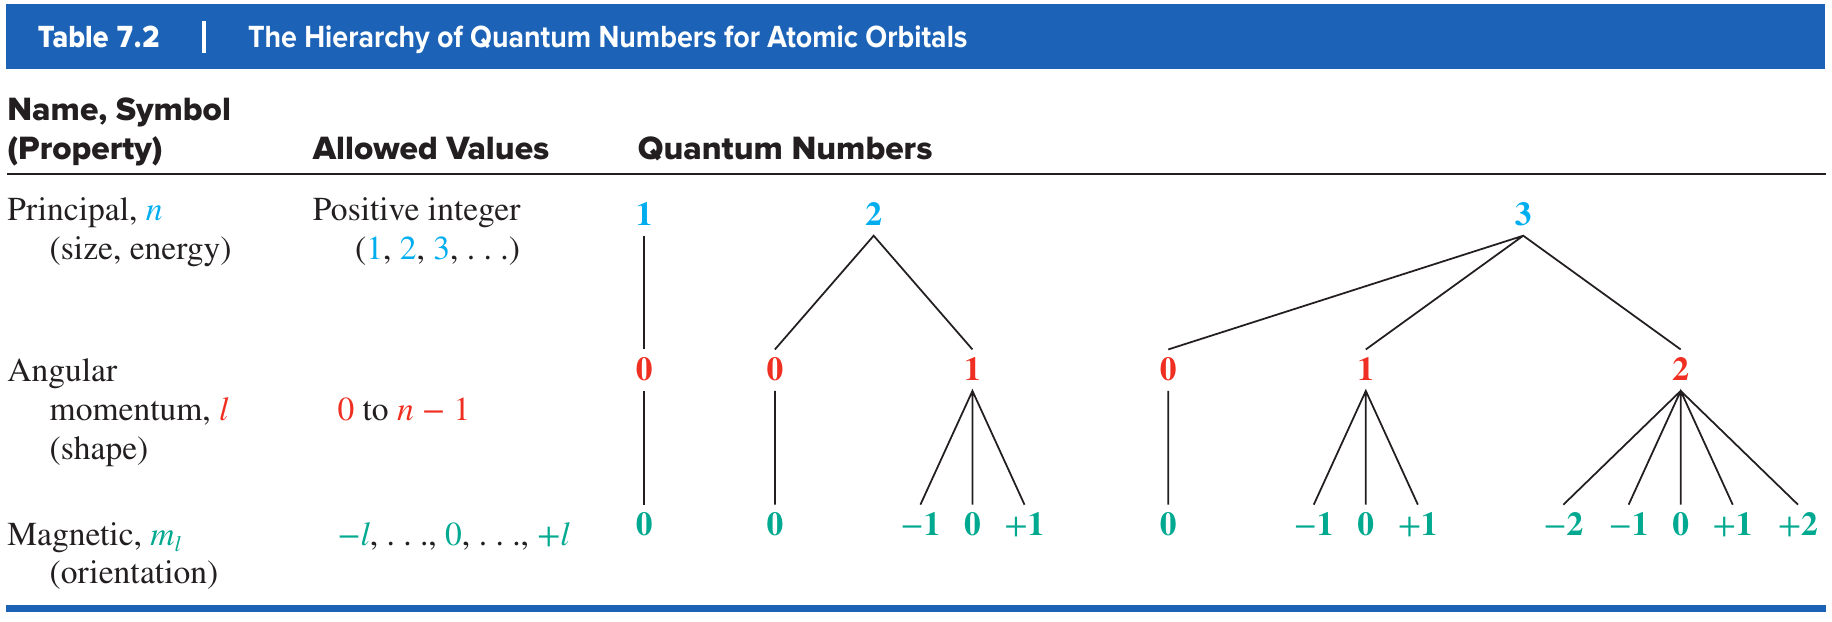
\includegraphics[width=12cm]{figuras/fig46}
      \end{center}
    
\end{frame}



  
%%%%%%%%%%%%%%%%  SLIDE 49 %%%%%%%%%%%%%%%%%%%%%%%%%%


\begin{frame} 
  \frametitle{Átomo de Hidrogênio}
  
  
      \begin{center}
        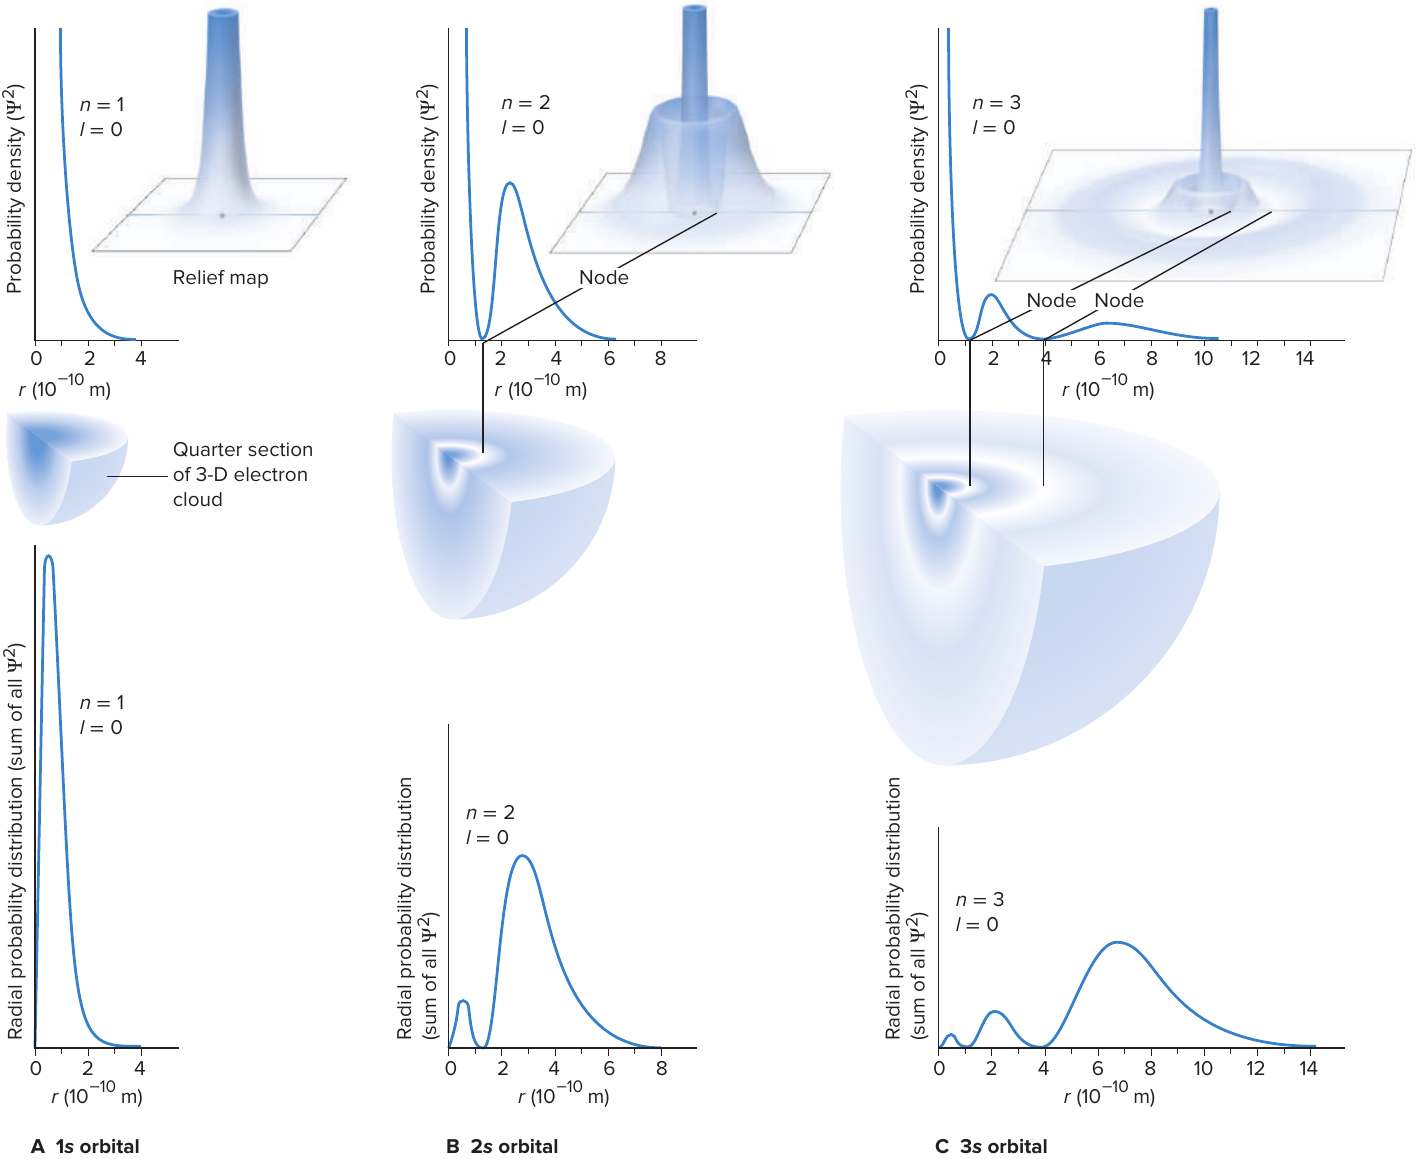
\includegraphics[height=8cm]{figuras/fig44}
      \end{center}
    
\end{frame}


%%%%%%%%%%%%%%%%  SLIDE 50 %%%%%%%%%%%%%%%%%%%%%%%%%%


\begin{frame} 
  \frametitle{Átomo de Hidrogênio}
  \fontsize{10pt}{11pt}\selectfont
  
  
      \begin{center}
        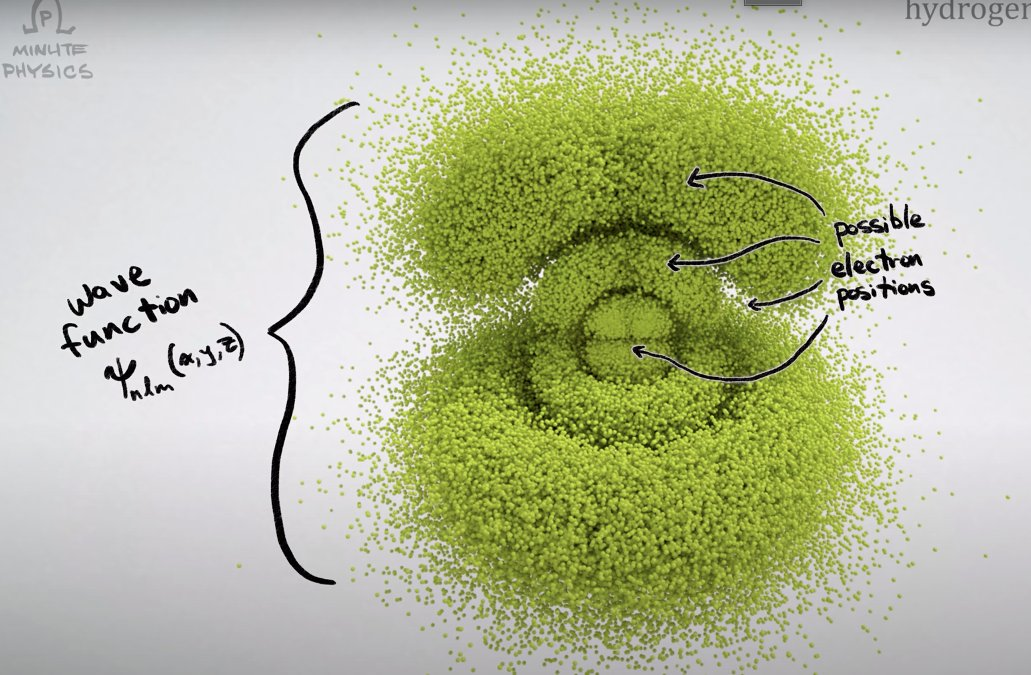
\includegraphics[height=6cm]{figuras/fig45}
      \end{center}
      
      \href{https://www.youtube.com/watch?v=W2Xb2GFK2yc}{\color{blue} Simulação do átomo de hidrogênio em base a teoria de De Broglie - Bohm}
    
\end{frame}


  
%%%%%%%%%%%%%%%%  SLIDE 43 %%%%%%%%%%%%%%%%%%%%%%%%%%


\begin{frame}
  \frametitle{Momento angular}
  \fontsize{7pt}{11pt}\selectfont

  
  \begin{columns}[T]

    \column{0.49\linewidth}
   Classicamente o momento angular está definido como
   \vspace*{-0.5cm}
   \begin{align*}
            \mathbf{L} &= \mathbf{r} \times \mathbf{p}\\
            &= \begin{vmatrix}
              \mathbf{i} & \mathbf{j} & \mathbf{k}\\
              x & y & z\\
              p_x & py & pz
            \end{vmatrix}\\
            &= \left( yp_z - zp_y \right)\,\mathbf{i} + \left( zp_x - xp_z \right)\,\mathbf{j} + \left( xp_y - yp_x \right)\,\mathbf{k}\\
            &= L_x\,\mathbf{i} +L_y \,\mathbf{j} +L_z \,\mathbf{k}
    \end{align*}
    
    utilizando o fato de que em quântica $\mathbf{p} = -i\hbar \nabla$ podemos esperar que par quântica
    
    \[
     \begin{align*}
            L_x &= -i\hbar\left( y \dfrac{\partial \;}{\partial z}  - z \dfrac{\partial \;}{\partial y}\right)\\
            L_y &= -i\hbar\left( z \dfrac{\partial \;}{\partial x}  - x \dfrac{\partial \;}{\partial z}\right)\\
            L_z &= -i\hbar\left( x \dfrac{\partial \;}{\partial y}  - y \dfrac{\partial \;}{\partial x}\right)\\
          \end{align*}
    \]
          
    passando para coordenadas esféricas
  
    \column{0.49\linewidth}
    \vspace*{-1cm}
    
    \begin{align*}
            L_x &= i\hbar \left( \sin \phi \dfrac{\partial \;}{\partial \theta} + \cos \phi \cot \theta \dfrac{\partial \;}{\partial \phi}\right)\\
            L_y &= i\hbar \left( -\cos \phi \dfrac{\partial \;}{\partial \theta} + \sin \phi \cot \theta \dfrac{\partial \;}{\partial \phi}\right)\\
            L_z &= -i\hbar\dfrac{\partial \;}{\partial \phi}
          \end{align*}
    de forma que podemos escrever (utilizando algumas identidades trigonométricas
    \[
     L^2 = -\hbar^2\left( \dfrac{1}{\sin \theta}\dfrac{\partial \;}{\partial \theta}\sin \theta \dfrac{\partial \;}{\partial \theta} + \dfrac{1}{\sin^2 \theta}\dfrac{\partial^2 \;}{\partial \phi^2}\right)
    \]
    equação que é igual à EDP da parte angular do átomo de hidrogênio, dessa analise podemos escrever
    \begin{align*}
     L^2 Y &= -\hbar^2\left( \dfrac{1}{\sin \theta}\dfrac{\partial \;}{\partial \theta}\sin \theta \dfrac{\partial \;}{\partial \theta} + \dfrac{1}{\sin^2 \theta}\dfrac{\partial^2 \;}{\partial \phi^2}\right)Y\\
     L^2 Y&=-\hbar^2 \lambda^2 Y\\
     L^2 Y&=l\left( l+1\right)\hbar Y
    \end{align*}
    
  \end{columns}
   
\end{frame}


  
%%%%%%%%%%%%%%%%  SLIDE 53 %%%%%%%%%%%%%%%%%%%%%%%%%%


\begin{frame}
  \frametitle{Teoria da medida}
  \fontsize{7pt}{11pt}\selectfont
  
  \setlength{\abovedisplayskip}{-8pt}
  \setlength{\belowdisplayskip}{2pt}
  \setlength{\abovedisplayshortskip}{-8pt}
  \setlength{\belowdisplayshortskip}{2pt}
  
  \begin{columns}[T]

    \column{0.49\linewidth}
%   Suponha que temos 2 operadores hermitianos $\hat{A}$ e $\hat{B}$ o qual significa que durante uma medida (valor esperado) um resultado possível será um do seus autovalores.
  
  A relação de dispersão em torno do valor medido é definido como
  
  \[
   \left( \Delta \hat{A}\right)^2 = \langle \hat{A}^2 \rangle - \langle \hat{A} \rangle^2
  \]

  Se escolhemos um sistema no qual $\langle \hat{A} \rangle=0$, então
  
  \[
   \left( \Delta \hat{A}\right)^2 = \langle \hat{A}^2 \rangle = \int\psi^*\hat{A}^2\psi dx =\langle\psi|\hat{A}^2|\psi\rangle
  \]
  
  o qual será verdade para operador $\hat{B}$. Usando a relação de Cauchy-Schwartz:
  
  \[
   \langle\psi|\hat{A}\hat{A}|\psi\rangle\langle\psi|\hat{B}\hat{B}|\psi\rangle \geqslant |\langle\psi|\hat{A}\hat{B}|\psi\rangle|^2
  \]

  do qual
  
  \[
  ({\Delta\hat{A}})^2({\Delta\hat{B}})^2 \geqslant |\langle\psi|\hat{A}\hat{B}|\psi\rangle|^2
  \]
  
  Agora, podemos reduzir o termo à direita
  
  \begin{align*}
    |\langle\psi|\hat{A}\hat{B}|\psi\rangle| & \geqslant  |Im\Big[\langle\psi|\hat{A}\hat{B}|\psi\rangle  \Big]\\
    & \geqslant \Big|\frac{1}{2i}\Big[\langle\psi|\hat{A}\hat{B}|\psi\rangle - \langle\psi|\hat{A}\hat{B}|\psi\rangle^*  \Big]\Big|
  \end{align*}

  já que o módulo de um número complexo é maior que sua parte imaginária. Além disso,
  
  \[
   f= Re(f)+i Im(f) \Rightarrow Im(f)=\frac{1}{2i}(f-f^*)
  \]

  \column{0.49\linewidth}
  
  Como $\hat{A}$ e $\hat{B}$ são observáveis então
  
  \[
   \langle\psi|\hat{A}\hat{B}|\psi\rangle^*=\langle\psi|(\hat{A}\hat{B})^{\dagger}|\psi\rangle=\langle\psi|(\hat{B}\hat{A})|\psi\rangle
  \]
  
  finalmente, utilizando este resultado podemos reescrever a inequação como
  
  \begin{align*}
   ({\Delta\hat{A}})^2({\Delta\hat{B}})^2 & \geqslant \Big|\frac{1}{2i}\Big[\langle\psi|\hat{A}\hat{B}\Big|\psi\rangle - \langle\psi \Big|\hat{B}\hat{A}\Big|\psi\rangle \Big]\Big|\\
   &\geqslant \Big|\frac{1}{2i}\Big[\langle\hat{A}\hat{B}\rangle - \langle\hat{B}\hat{A}\rangle \Big] \Big|\\
   &\geqslant \Big|\frac{1}{2i}\langle[\hat{A},\hat{B}]\rangle\Big|
  \end{align*}

  de forma que a relação de dispersão para qualquer par de operadores hermitiano está relacionado com seu comutador via
  
  \[
   ({\Delta\hat{A}})^2({\Delta\hat{B}})^2 \geqslant \Big|\frac{1}{2i}\langle[\hat{A},\hat{B}]\rangle \Big|
  \]

  ou seja, se dois operadores comutam então podem ser medidos simultaneamente com precisão absoluta, caso não comutem a precisão da medida tem uma cota superior
   
  \end{columns}
\end{frame}



  
%%%%%%%%%%%%%%%%  SLIDE 53 %%%%%%%%%%%%%%%%%%%%%%%%%%


\begin{frame}
  \frametitle{Momento angular}
  \fontsize{7pt}{11pt}\selectfont
  
  \setlength{\abovedisplayskip}{-8pt}
  \setlength{\belowdisplayskip}{2pt}
  \setlength{\abovedisplayshortskip}{-8pt}
  \setlength{\belowdisplayshortskip}{2pt}

  
  \begin{columns}[T]
    \column{0.49\linewidth}
      As componentes do momento angular não comutam entre sim
      
      \[
       \left[x_i,\,p_j\right] = i\hbar \delta_{ij}
      \]
      
      \begin{align*}
        \left[ L_x,\, L_y\right] &= \left[ \left( yp_z - zp_y \right), \left( zp_x - xp_z \right)  \right]\\
            &=  \left[ yp_z ,\, zp_x  \right] - \left[ yp_z ,\,  xp_z\right] -\left[ zp_y ,\, zp_x \right]\, + \left[ zp_y ,\, xp_z \right]
      \end{align*}
      
      como
      
      \begin{align*}
            \left[ yp_z ,\,  xp_z\right] &= \left[ y ,\,  x\right]p_z=0\\
            \left[ zp_y ,\, zp_x \right] &= z\left[ p_y ,\, p_x \right]=0\\
            \left[ yp_z ,\, zp_x  \right] &= yp_z\, zp_x - zp_x\, yp_z\\
            &= yp_z\, p_xz - zy\,p_xp_z\\
            &= yp_x\, p_zz - yz\,p_xp_z\\
            &= yp_x\, p_zz - yp_x\,zp_z\\
            &= yp_x\left( p_zz - zp_z \right)\\
            &= yp_x\left[ p_z ,\, z \right]\\
            &= -i\hbar yp_x
          \end{align*}
          


    \column{0.49\linewidth}
      então
      
        \begin{align*}
            \left[ L_x,\, L_y\right] &= i\hbar\left( xp_y -  yp_x\right)\\
            &= iL_z
          \end{align*}
          
      da mesma forma
      
      \begin{align*}
            \left[ L_y,\, L_z\right] &= iL_x\\
            \left[ L_z,\, L_x\right] &= iL_y
          \end{align*}
          
      Por outro lado, é possível verificar
      
      \begin{align*}
            \left[ L^2 ,\, L_z \right] &= \left[ L_x^2 ,\, L_z \right] + \left[ L_y^2 ,\, L_z \right]\\
            &\quad + \left[ L_z^2 ,\, L_z \right]
          \end{align*}
          
      de forma que os harmônicos esféricos que são autofunções de 
      $L^2$ também são autofunções de \\
      $L_z$. Por definição
      
      \begin{align*}
            L_z &= -i\hbar \dfrac{\partial \;}{\partial \phi}\\
            L_z^2 &= -\hbar^2 \dfrac{\partial^2 \;}{\partial \phi^2}\\
            L_z^2\Phi &= -\hbar^2 \dfrac{\partial^2 \Phi}{\partial \phi^2}
          \end{align*}
  \end{columns}

\end{frame}

% 
% %%%%%%%%%%%%%%%%  SLIDE 53 %%%%%%%%%%%%%%%%%%%%%%%%%%
% 
% 
% \begin{frame}
%   \frametitle{Momento angular}
%   \fontsize{7pt}{11pt}\selectfont
%   
%   Como $\Phi(\phi) = \dfrac{1}{\sqrt{2\pi}}\exp\left(im\phi\right)$, então
%   
%   \[
%    L_z^2\Phi_m = m^2\hbar^2\Phi_m
%   \]
%   
%   e como $Y=\Theta(\theta) \Phi(\phi)$, então
%   
%   \[
%    L_z^2Y_{lm} = m^2\hbar^2Y_{lm}
%   \]
% 
%   o que implica que tanto $L^2$ quanto $L_z^2$ podem ser determinados simultaneamente. 
%   
%   
%   A não comutação das componentes de $L$ implica na impossibilidade de se poder determinar a posição exata do vetor momento angular. O que podemos determinar é a direção de uma da suas componentes (chamada de $L_z$) e ignorar as outras
% 
% 
% \end{frame}

\end{document}
